\documentclass{article}
\usepackage[utf8]{inputenc}
\usepackage[english]{babel}
\usepackage{lipsum}
\usepackage{amsmath,graphicx}%,supp}
\usepackage{hyperref}

% Change page margins
% -------------------
\usepackage[a4paper, total={6.5in, 9in}]{geometry}

% Change default font to Times New Roman
% --------------------------------------
\usepackage{mathptmx}

% Page settings
% ---------------
\usepackage{lastpage}
\usepackage{fancyhdr}
% Uncomment to remove the header rule
%\renewcommand{\headrulewidth}{0pt} 
%\pagestyle{fancy}
%\fancyfoot[C]{Page \thepage\ of \pageref{LastPage}}
%\fancyhead[R]{02456 Deep Learning, Fall 2020}
\fancyhead[L]{Supplementary material}


% Captions as supplementary figures
% ---------------------------------
\usepackage[figurename=Fig.]{caption}
\usepackage[labelfont=bf]{caption}
\renewcommand{\thefigure}{S\arabic{figure}}
\renewcommand{\thetable}{S\arabic{table}}

% ----------- begin document -----------
\begin{document}
\section*{Supplementary material}


\begin{center}
  \textit{Note that the rest of analyses and results generated in this project can be found online on \href{https://github.com/laurasansc/02456_scVAE}{GitHub}.}  
\end{center}

% data set - tSNE
\begin{figure}[h!]
    \centering
    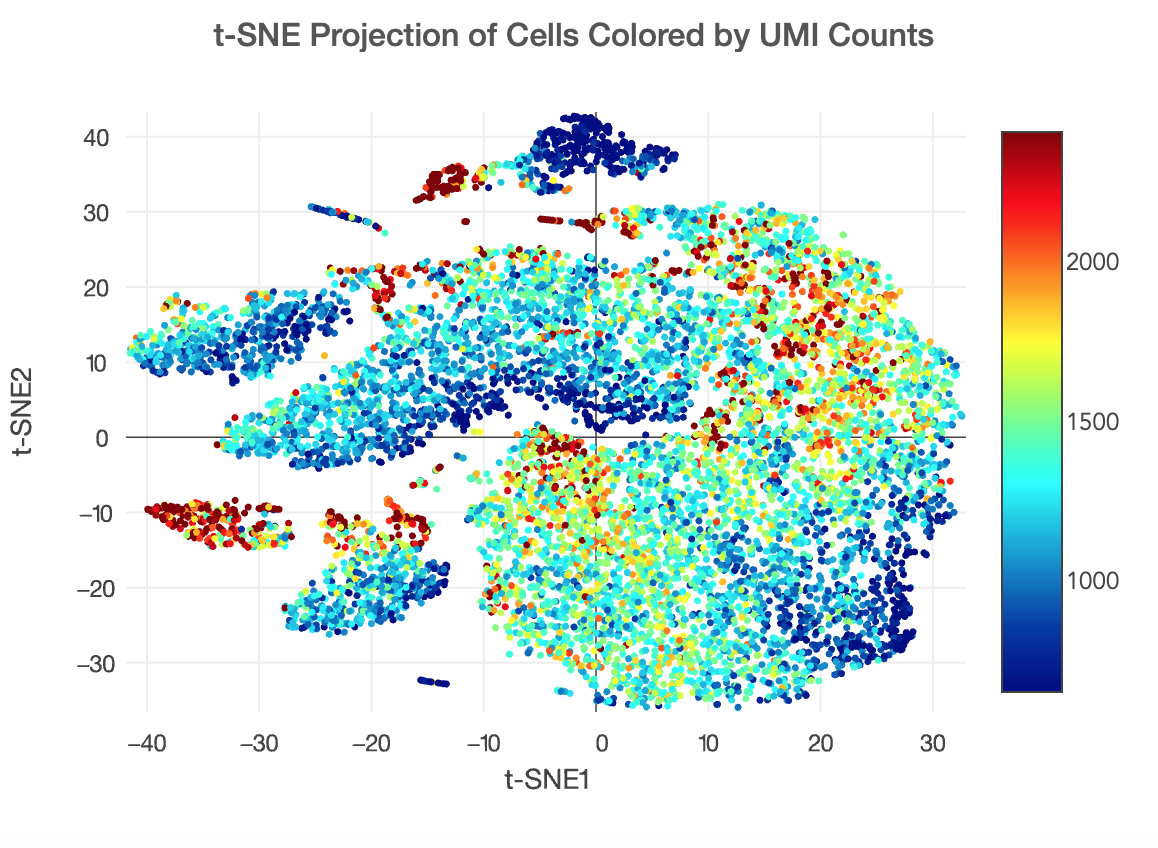
\includegraphics[width=0.49\textwidth]{02456_report/images/supp/tsne_umi.png}
    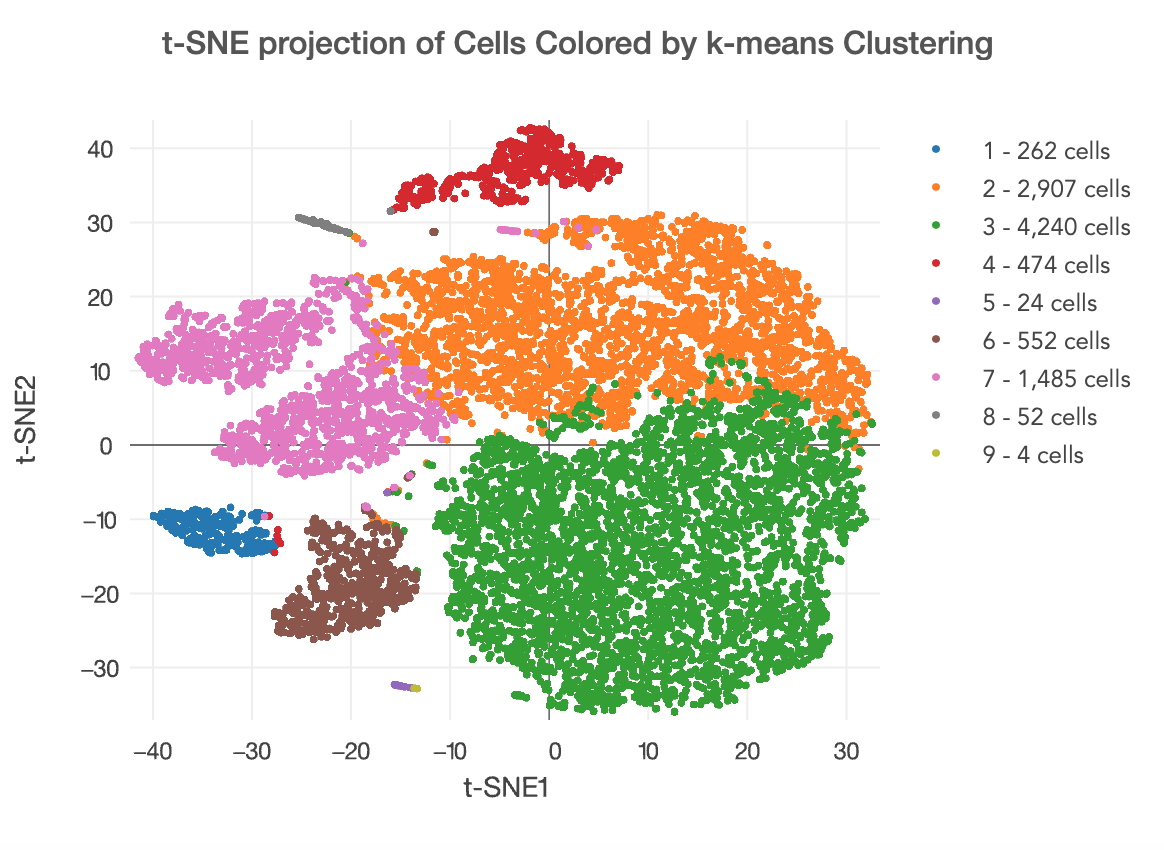
\includegraphics[width=0.49\textwidth]{02456_report/images/supp/tsne_cluster.png}
    \caption{t-SNE projections of the 10x-68k-PMBC data set, in the left colored by UMI counts and in the right, it shows the 68k cells clustered by K-means clustering. k numbers of clusters as 10. The plots are extracted from the summary released in 10X Genomics website.}
    %\href{https://cf.10xgenomics.com/samples/cell-exp/1.1.0/fresh_68k_pbmc_donor_a/fresh_68k_pbmc_donor_a_web_summary.html}{10X Genomics website}.
    \label{sfig:dataset}
\end{figure}

% pca - variance explained
\begin{figure}[h!]
    \centering
    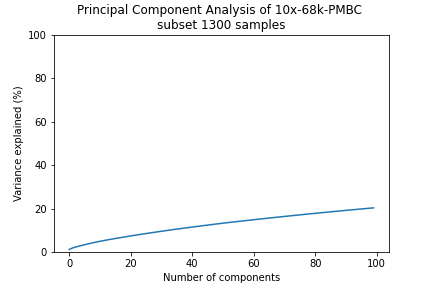
\includegraphics[width=0.70\textwidth]{02456_report/images/supp/pca.png}
    \caption{Variance explained over $k$ components resulting from applying PCA to the 2\% subset from 10x-68k-PMBC data.}
    \label{sfig:pca}
\end{figure} 

%% ------------------ FFNN -----------------

\begin{figure}[h!]
    \centering
    
\includegraphics[width=0.33\textwidth]{02456_report/images/supp/confusion_matrix_subset1300_raw.png}
    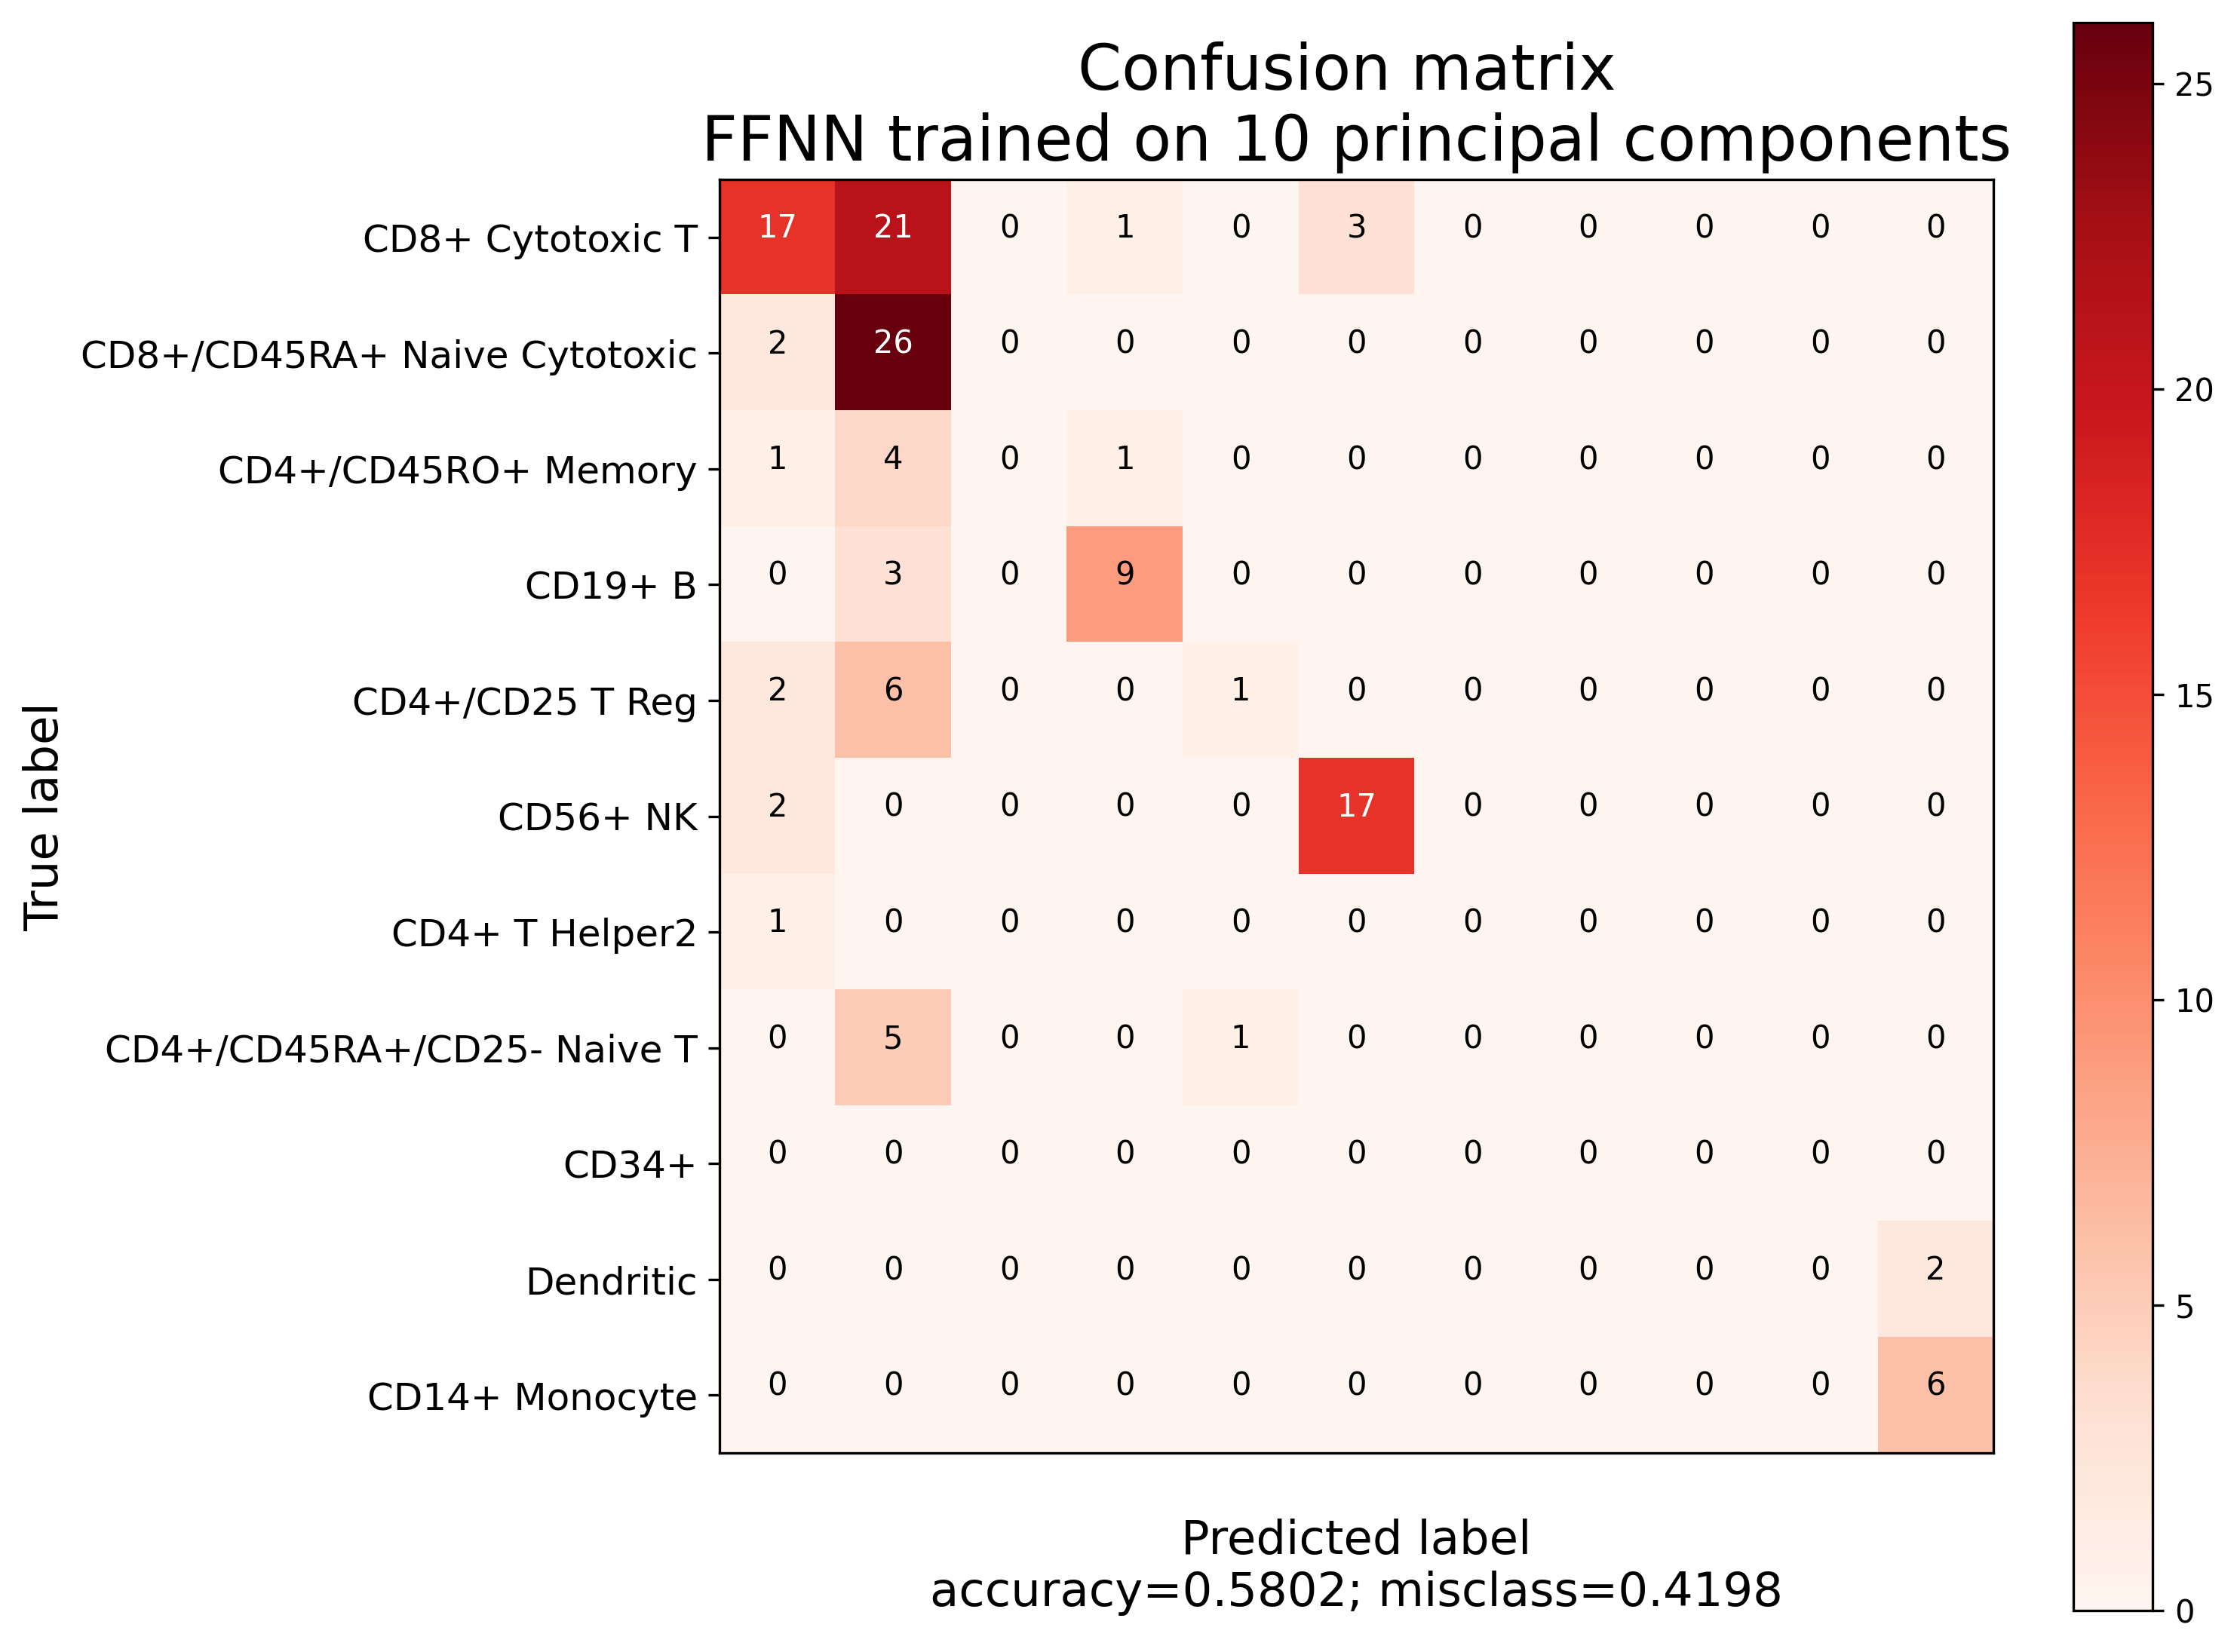
\includegraphics[width=0.33\textwidth]{02456_report/images/supp/confusion_matrix_subset1300_pca10.png}
    
\includegraphics[width=0.33\textwidth]{02456_report/images/supp/confusion_matrix_subset1300_pca25.png}
    
\includegraphics[width=0.33\textwidth]{02456_report/images/supp/confusion_matrix_subset1300_pca50.png}
    
\includegraphics[width=0.33\textwidth]{02456_report/images/supp/confusion_matrix_subset1300_pca100.png}
    
\includegraphics[width=0.33\textwidth]{02456_report/images/supp/confusion_matrix_subset1300_scvae10_H250.png}
    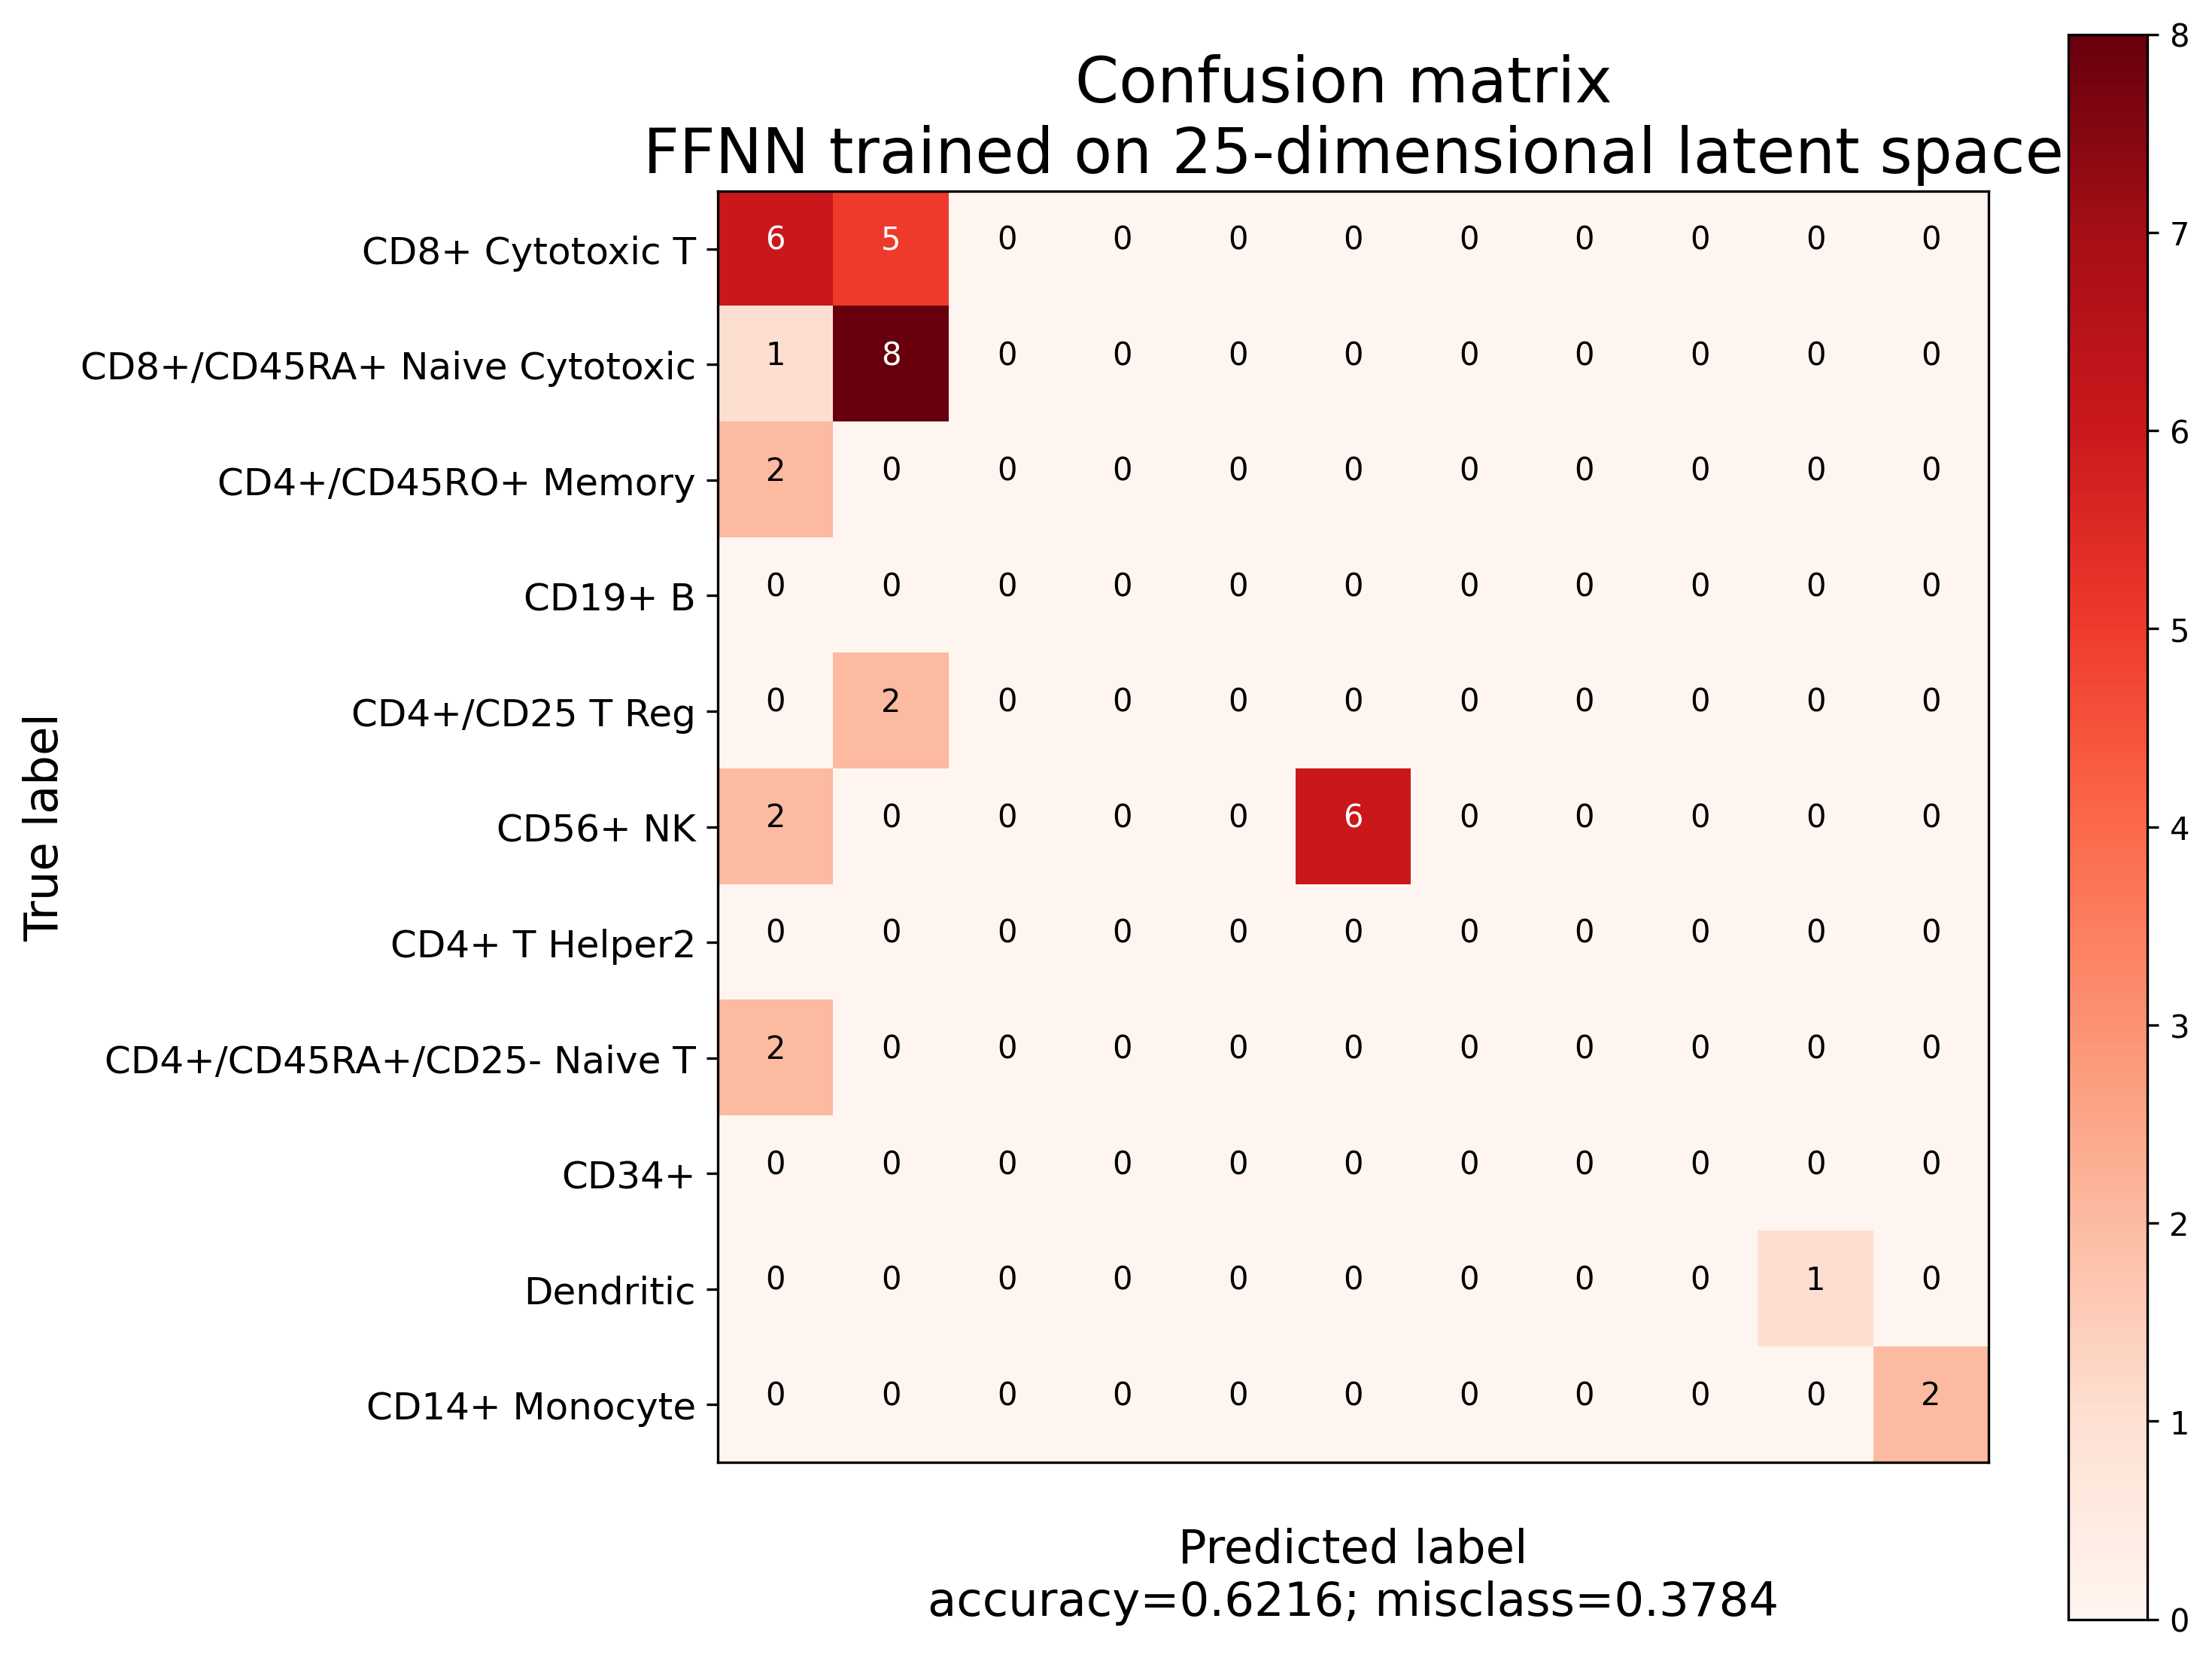
\includegraphics[width=0.33\textwidth]{02456_report/images/supp/confusion_matrix_subset1300_scvae25_H500.png}
    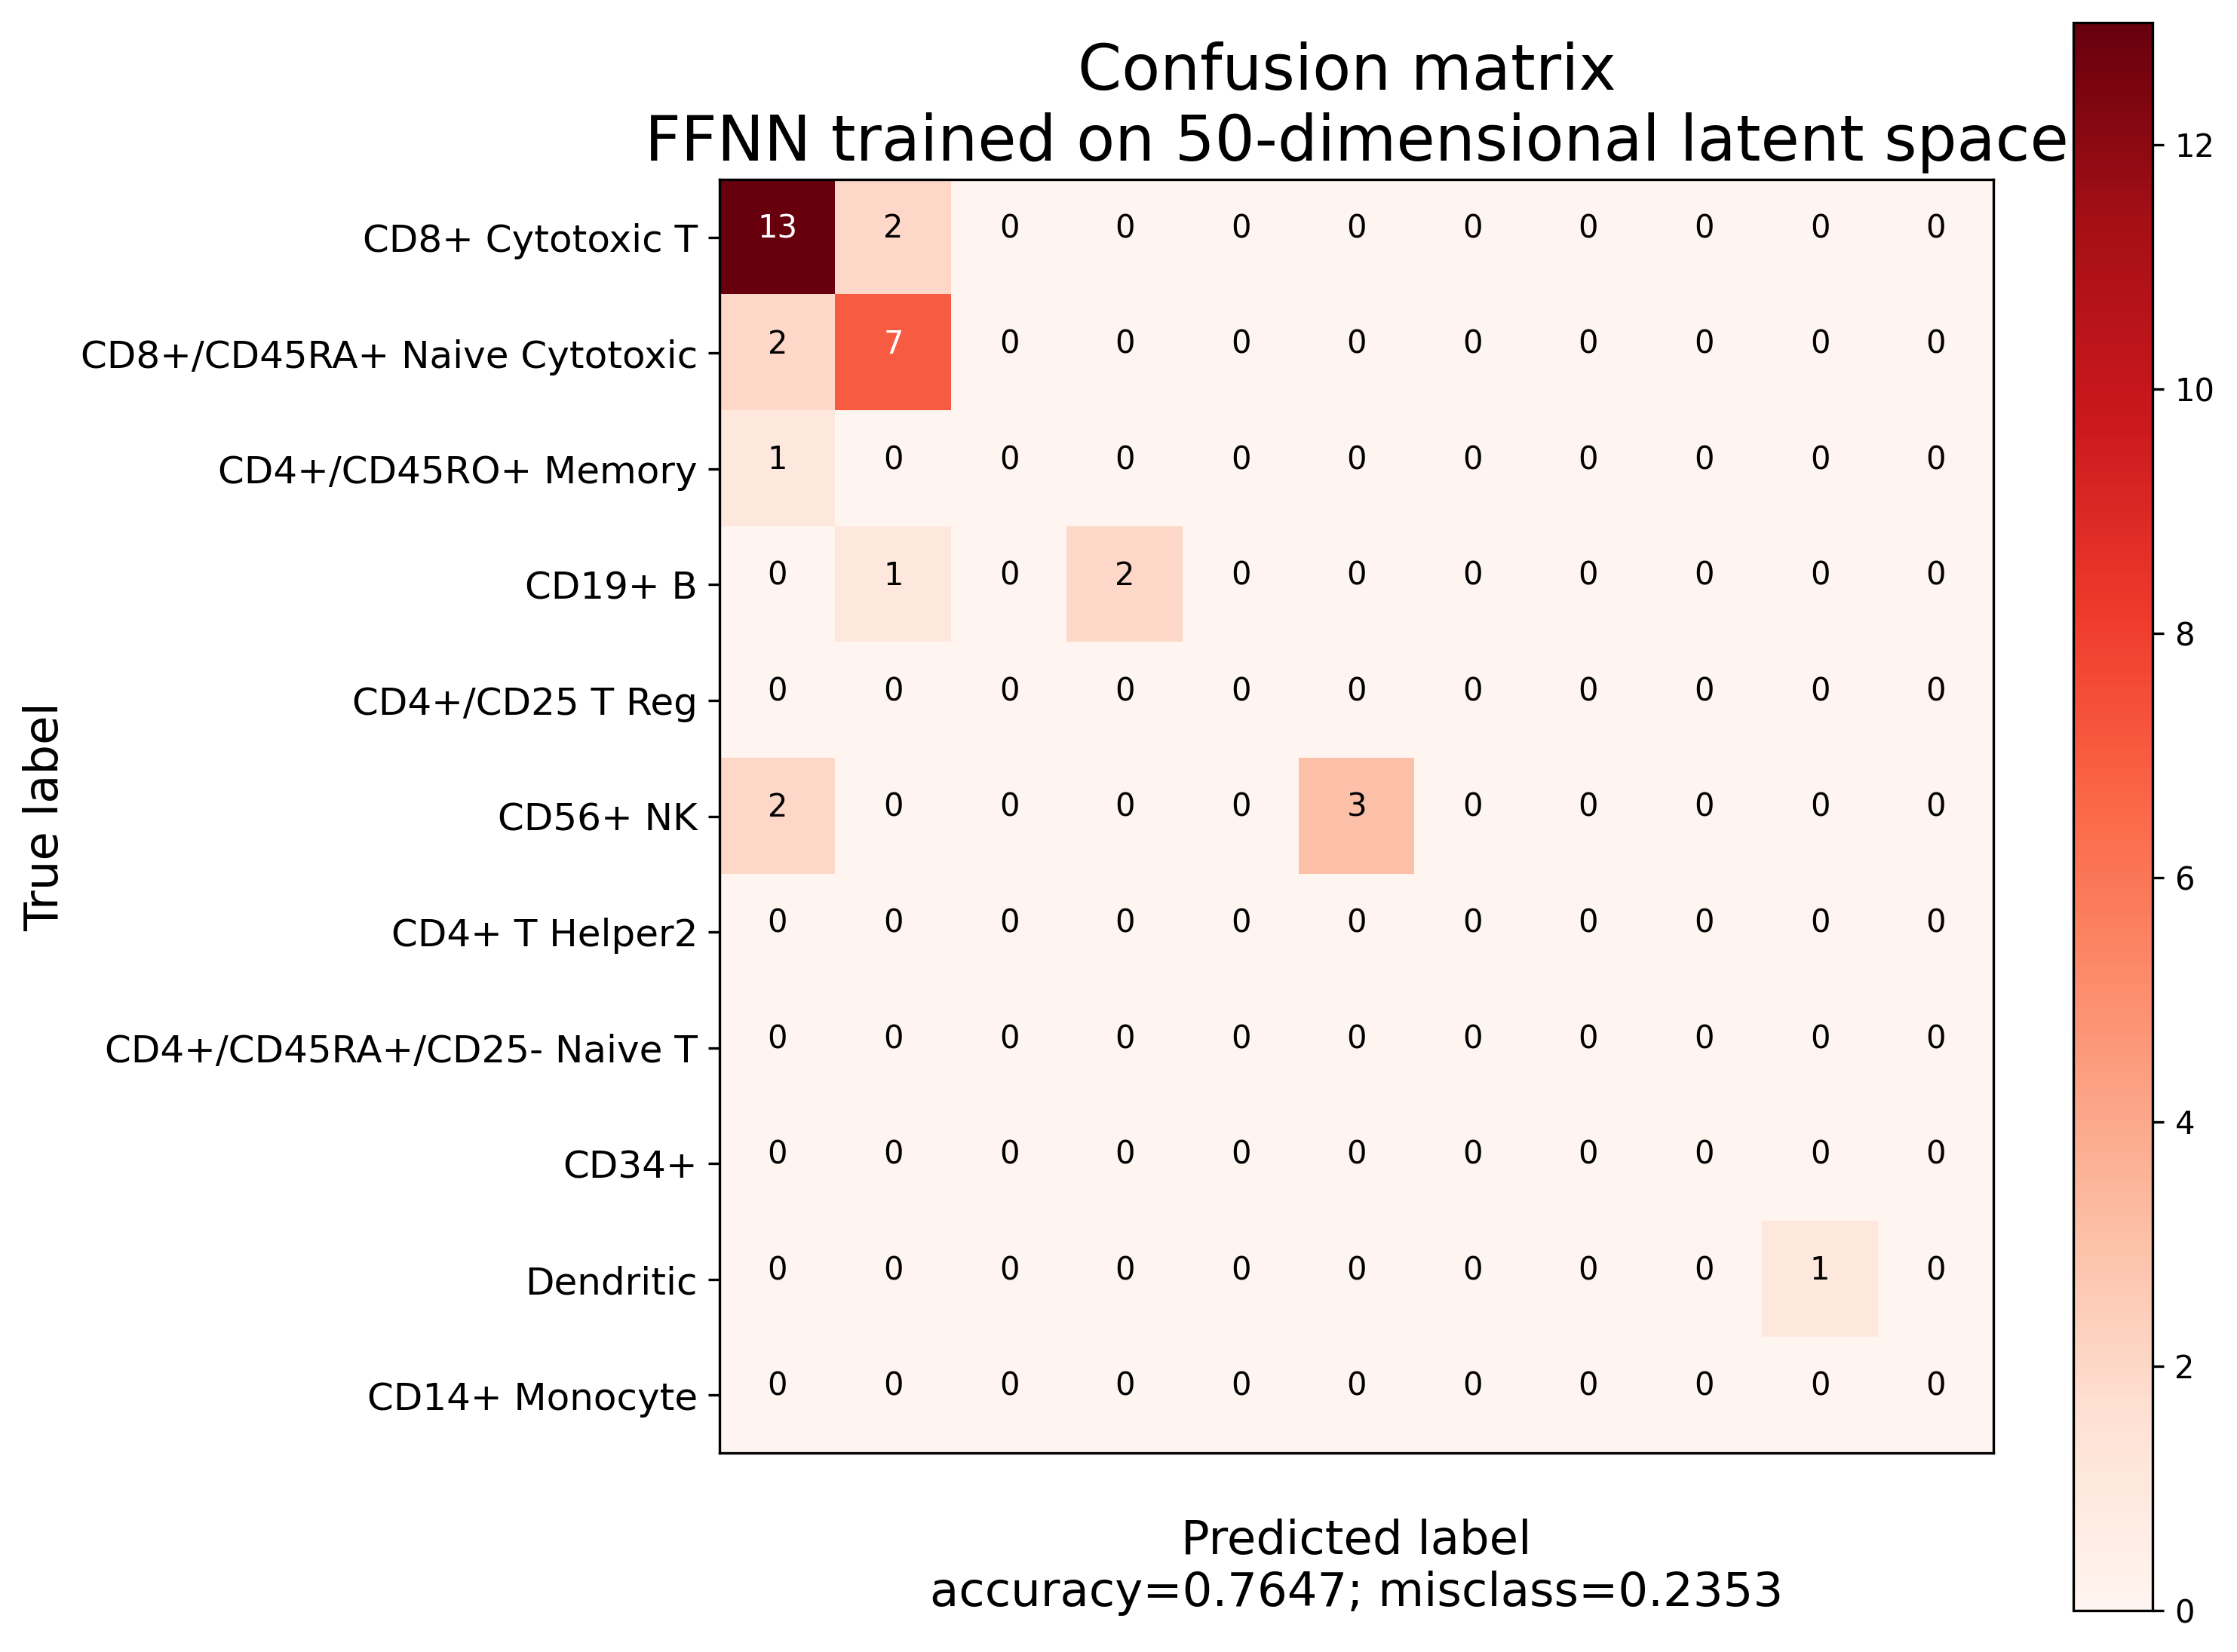
\includegraphics[width=0.33\textwidth]{02456_report/images/supp/confusion_matrix_subset1300_scvae50_H250.png}
    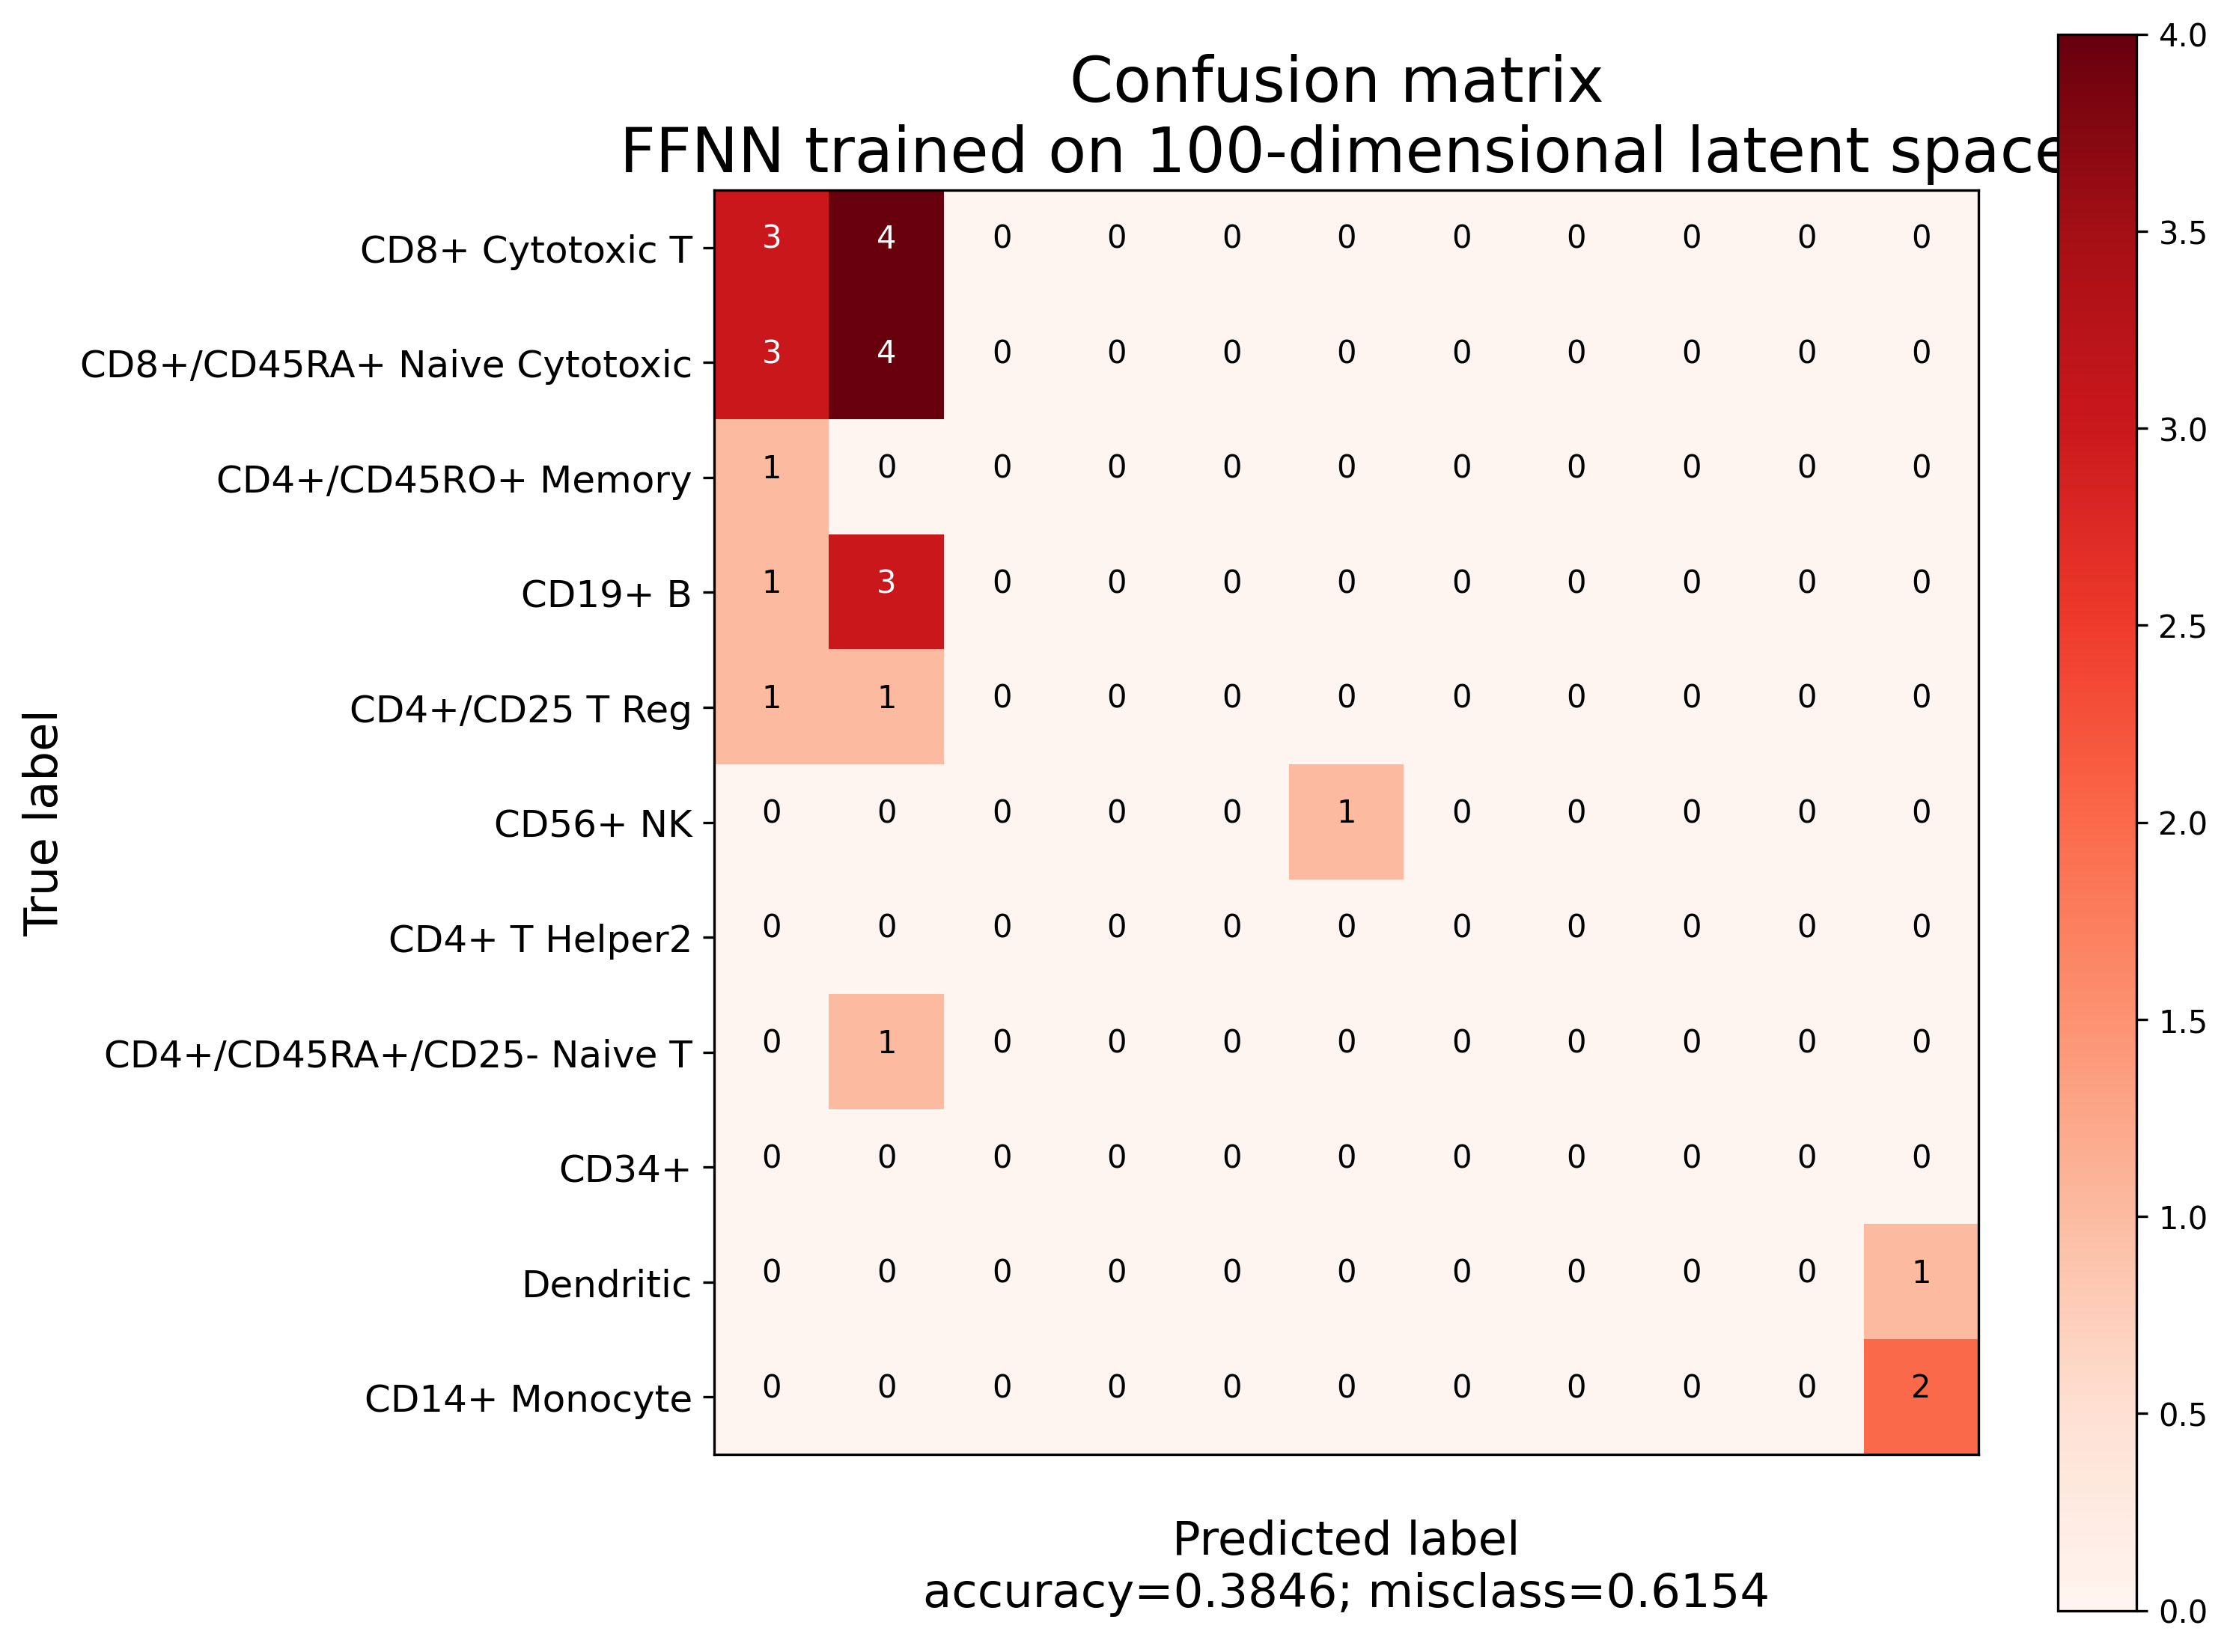
\includegraphics[width=0.33\textwidth]{02456_report/images/supp/confusion_matrix_subset1300_scvae100_H500.png}
    \caption{Confusion matrices from each FFNN model test set for the subset with 1,300 cells. }
    \label{sfig:confusions1300}
\end{figure}

\begin{figure}[h!]
    \centering
    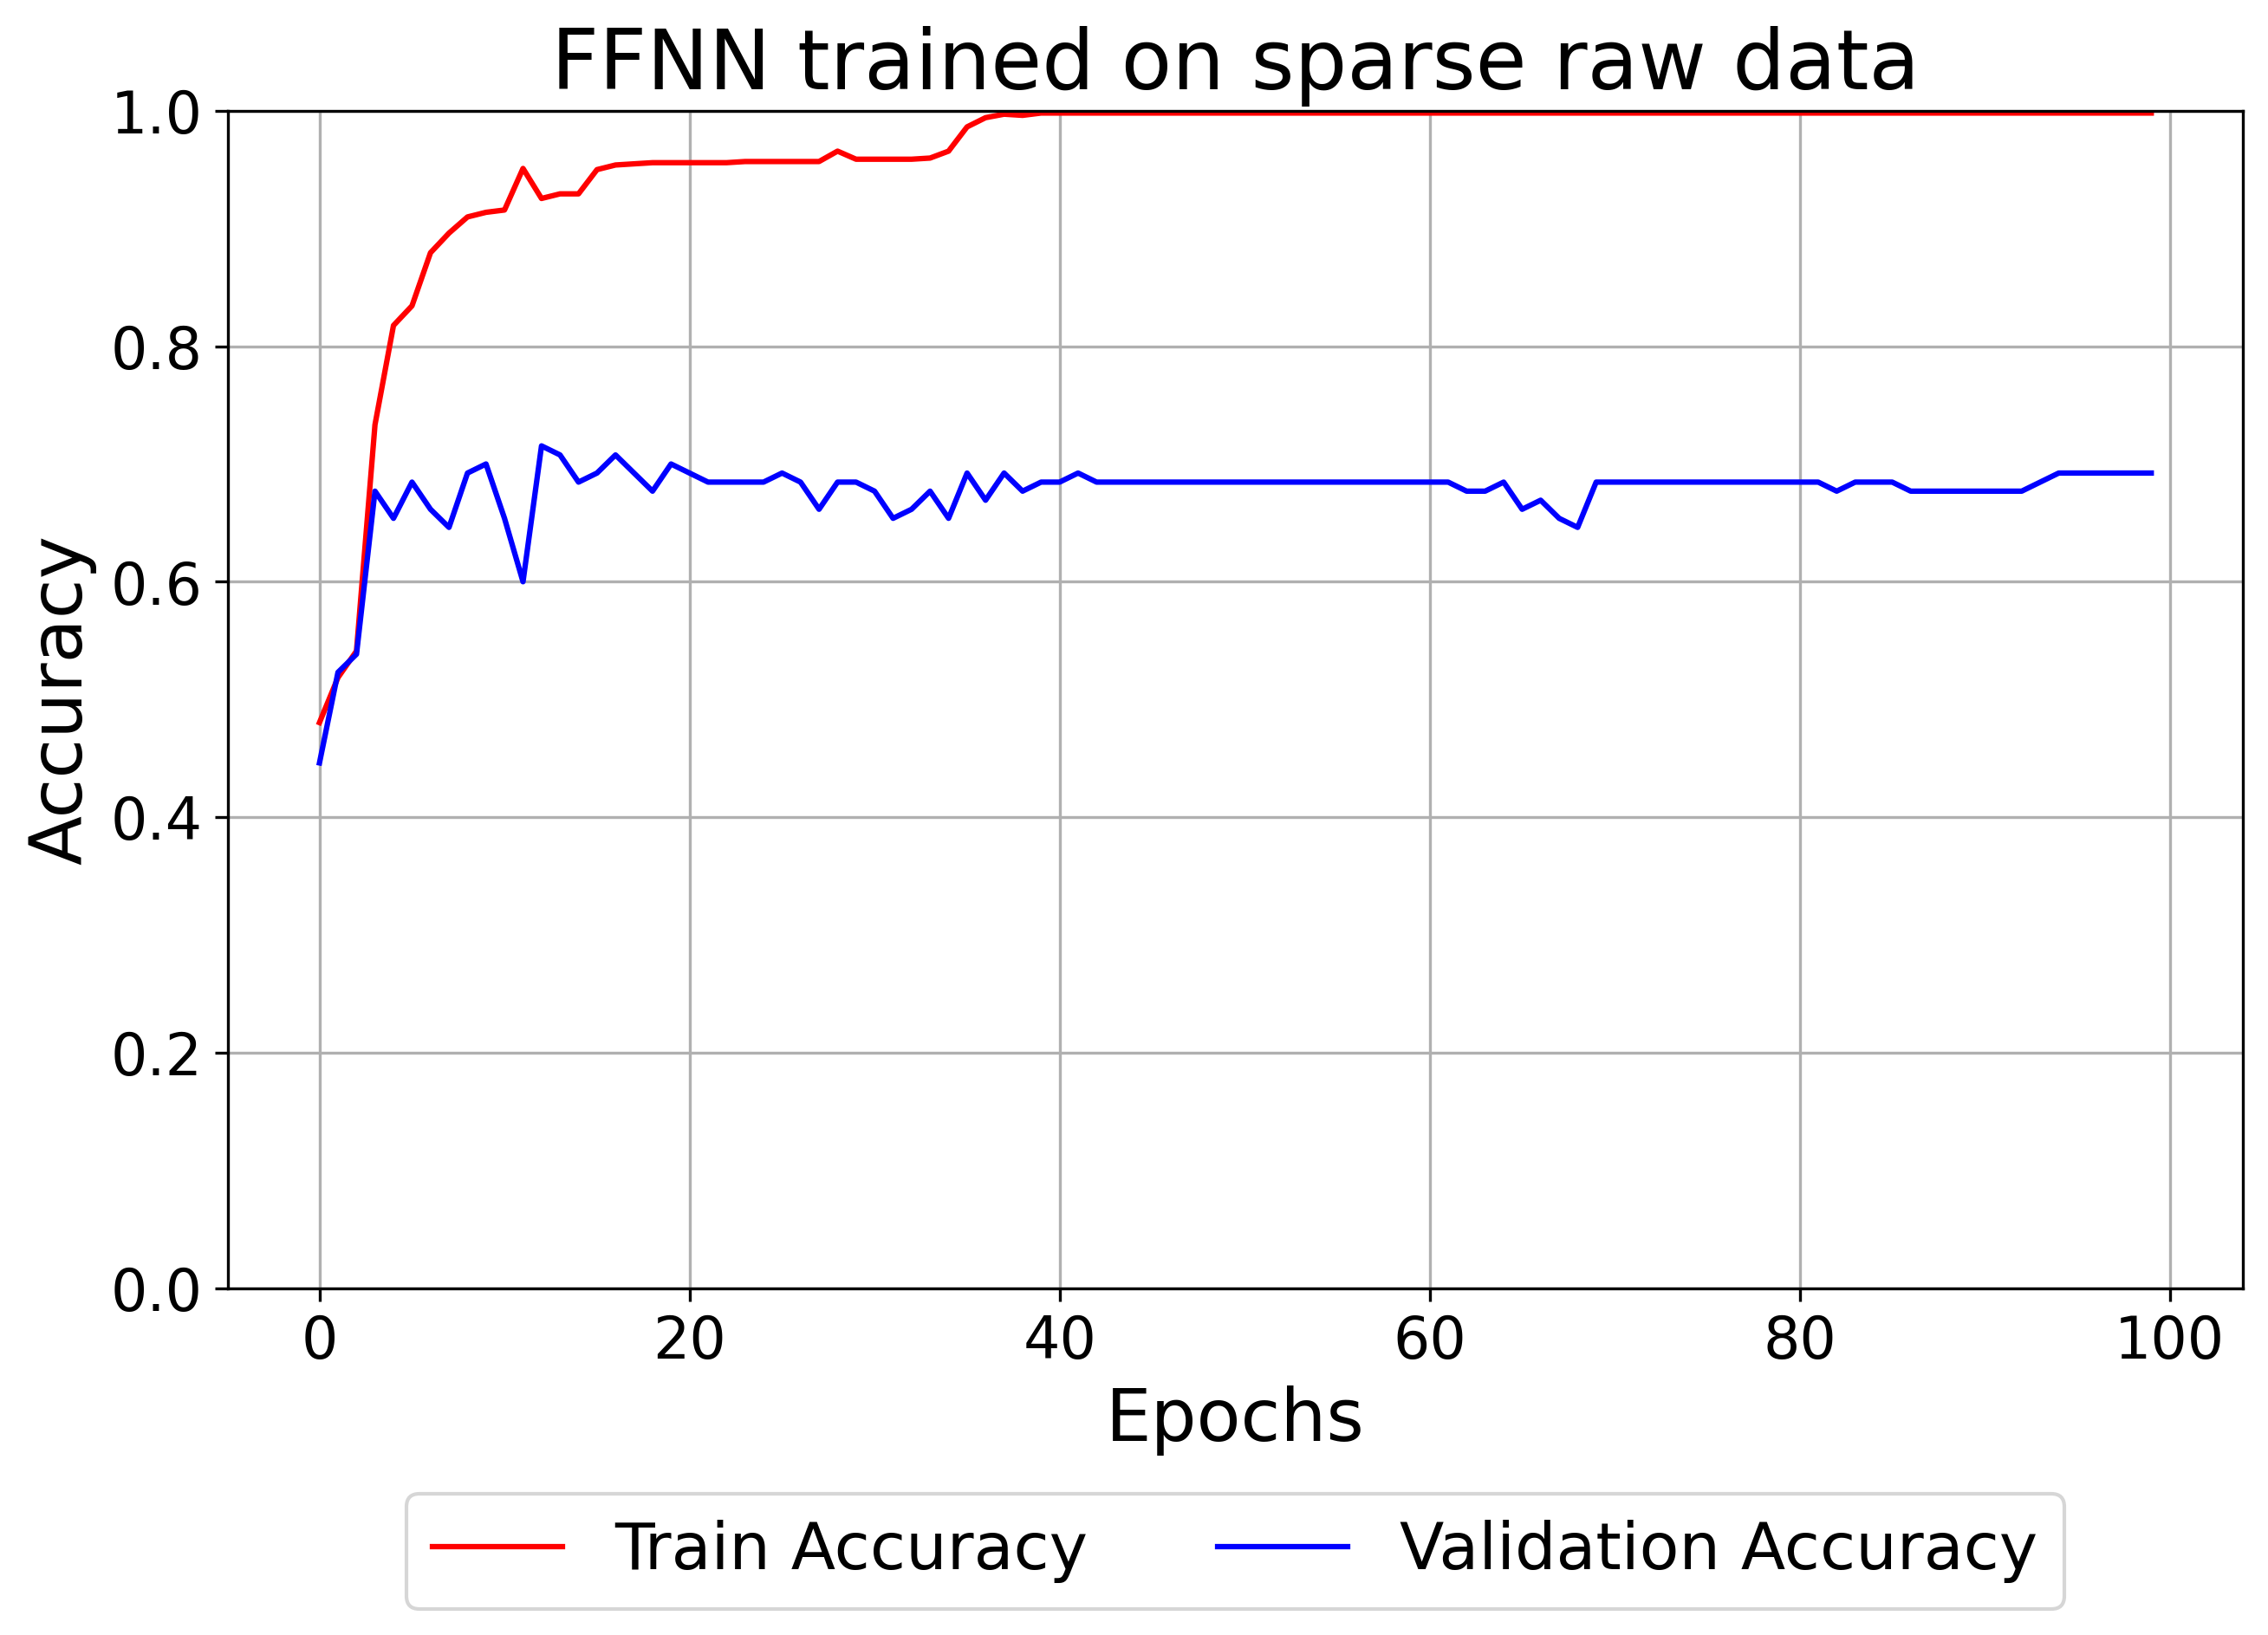
\includegraphics[width=0.33\textwidth]{02456_report/images/supp/learning_curve_subset1300_raw.png}
    
\includegraphics[width=0.33\textwidth]{02456_report/images/supp/learning_curve_subset1300_pca10.png}
    
\includegraphics[width=0.33\textwidth]{02456_report/images/supp/learning_curve_subset1300_pca25.png}
    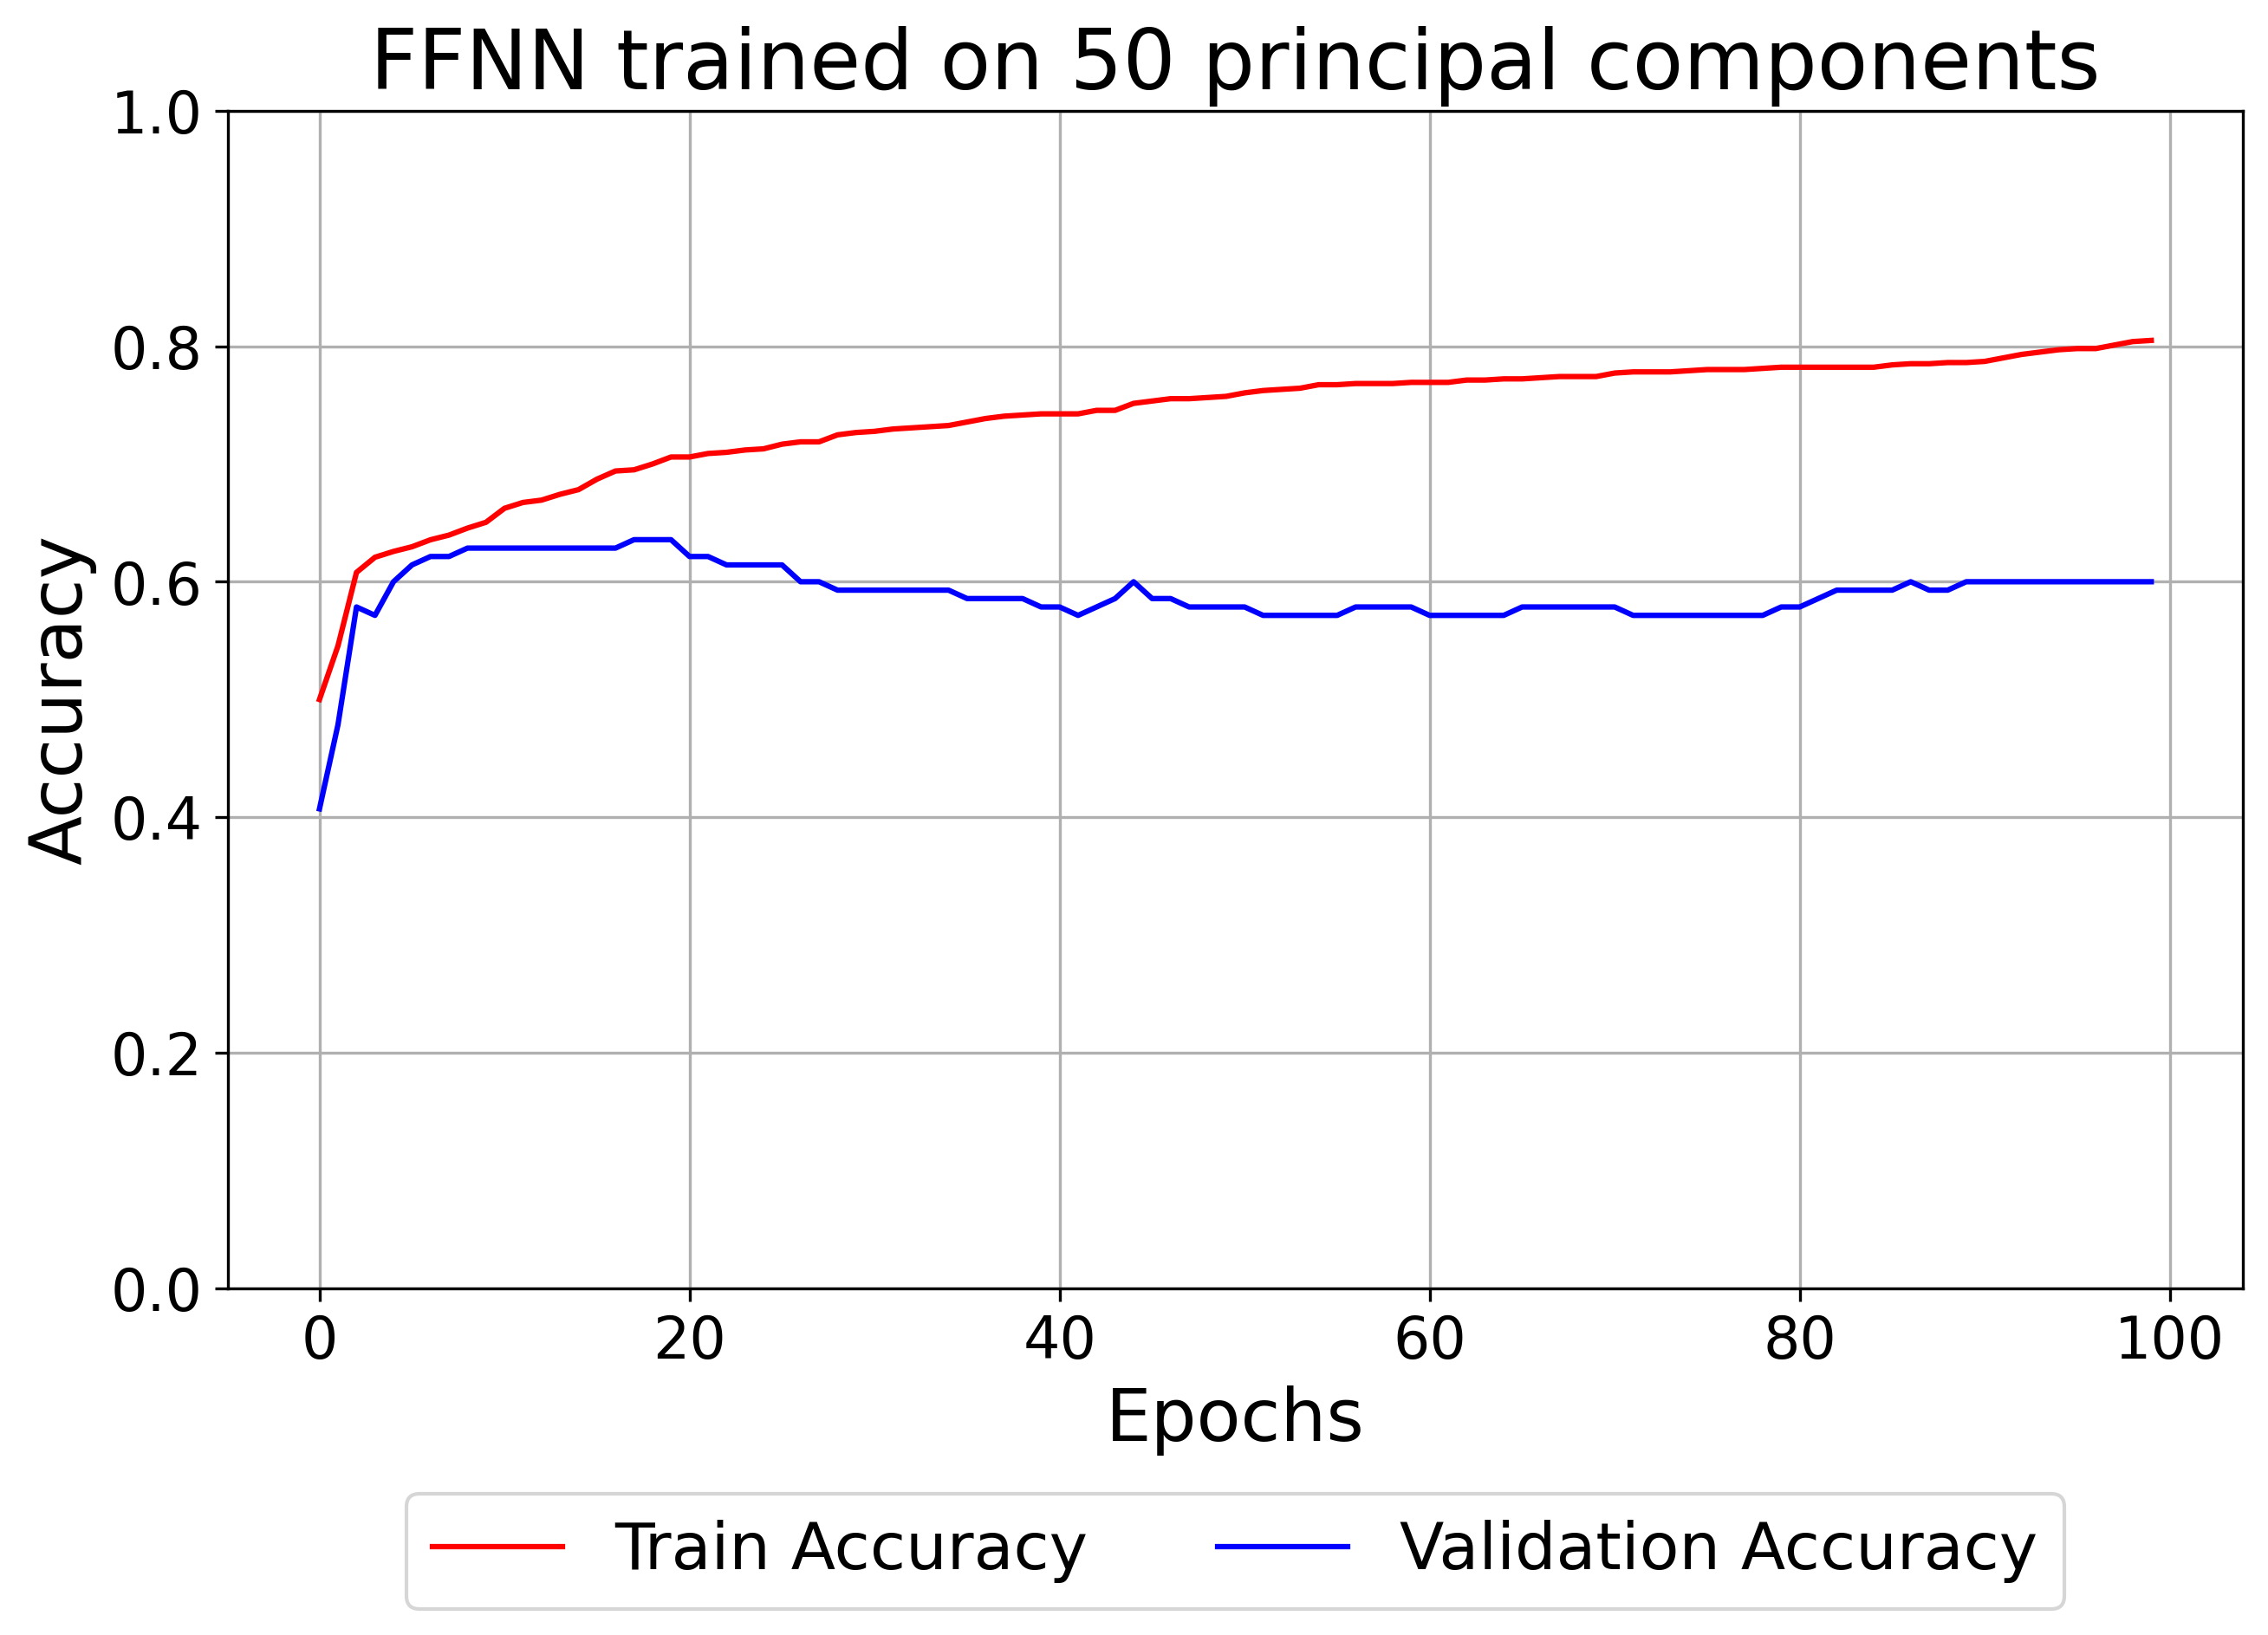
\includegraphics[width=0.33\textwidth]{02456_report/images/supp/learning_curve_subset1300_pca50.png}
    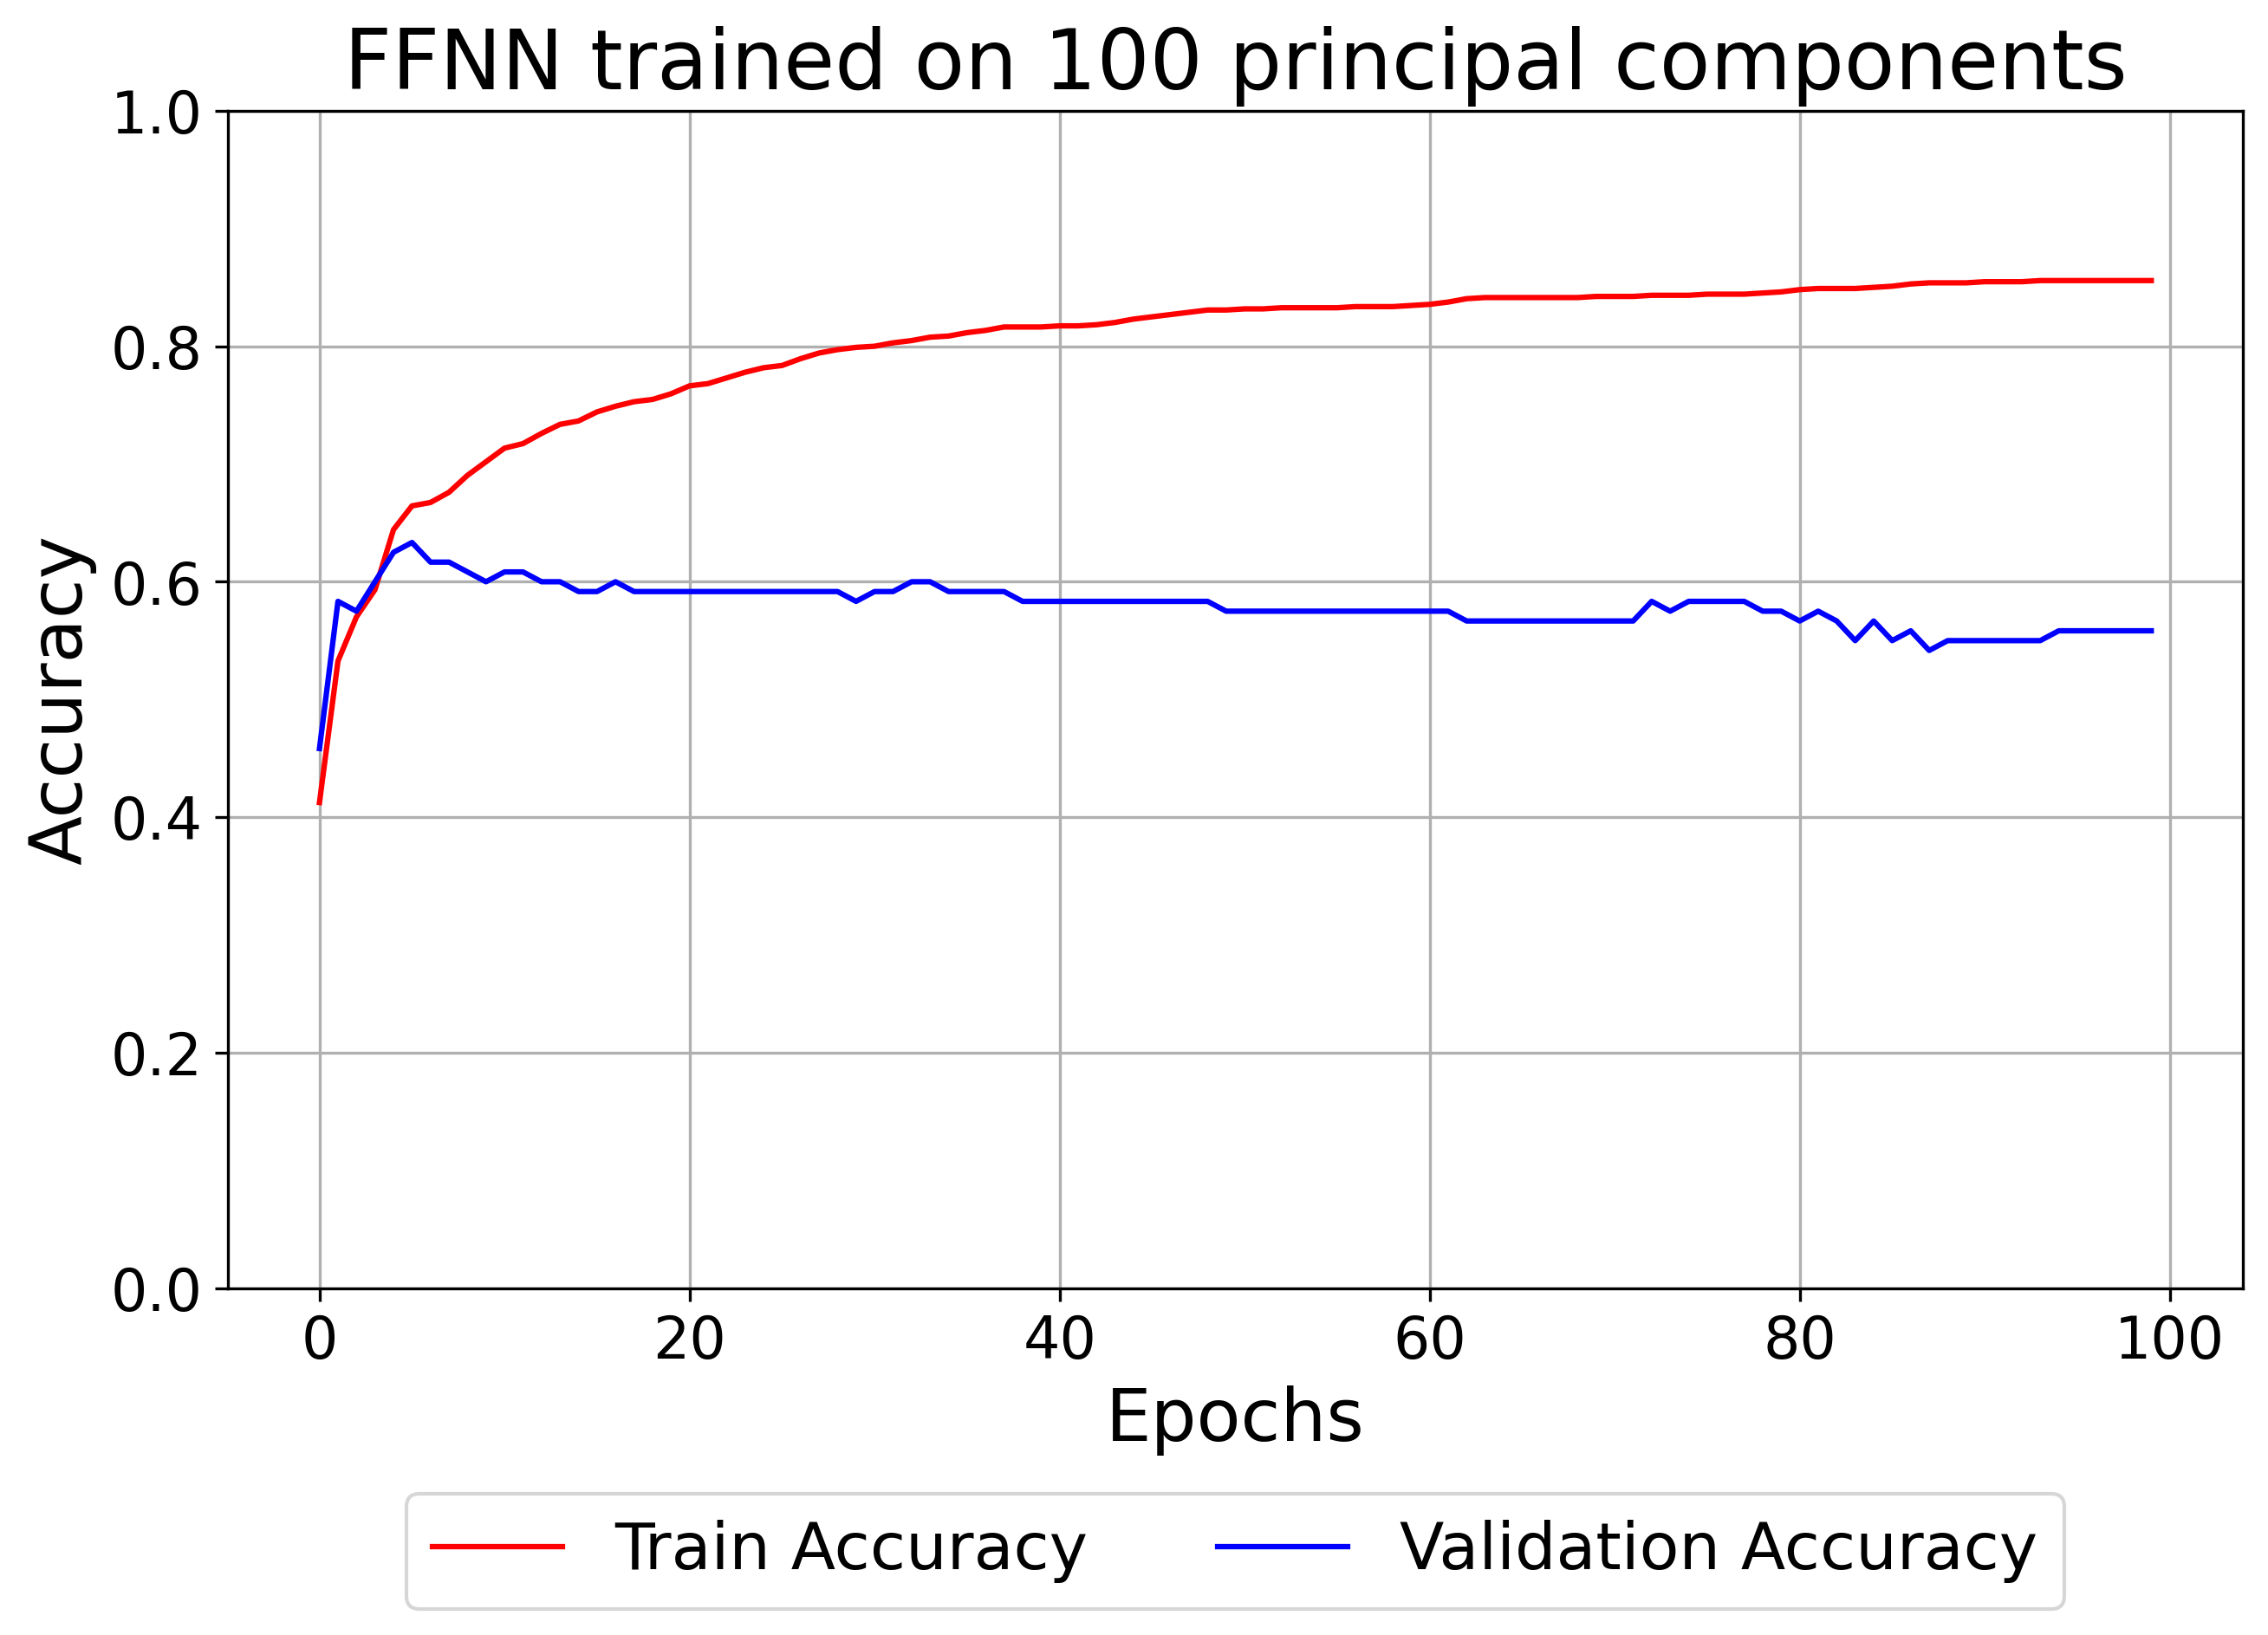
\includegraphics[width=0.33\textwidth]{02456_report/images/supp/learning_curve_subset1300_pca100.png}
    
\includegraphics[width=0.33\textwidth]{02456_report/images/supp/learning_curve_subset1300_scvae10_H250.png}
    
\includegraphics[width=0.33\textwidth]{02456_report/images/supp/learning_curve_subset1300_scvae25_H500.png}
    
\includegraphics[width=0.33\textwidth]{02456_report/images/supp/learning_curve_subset1300_scvae50_H250.png}
    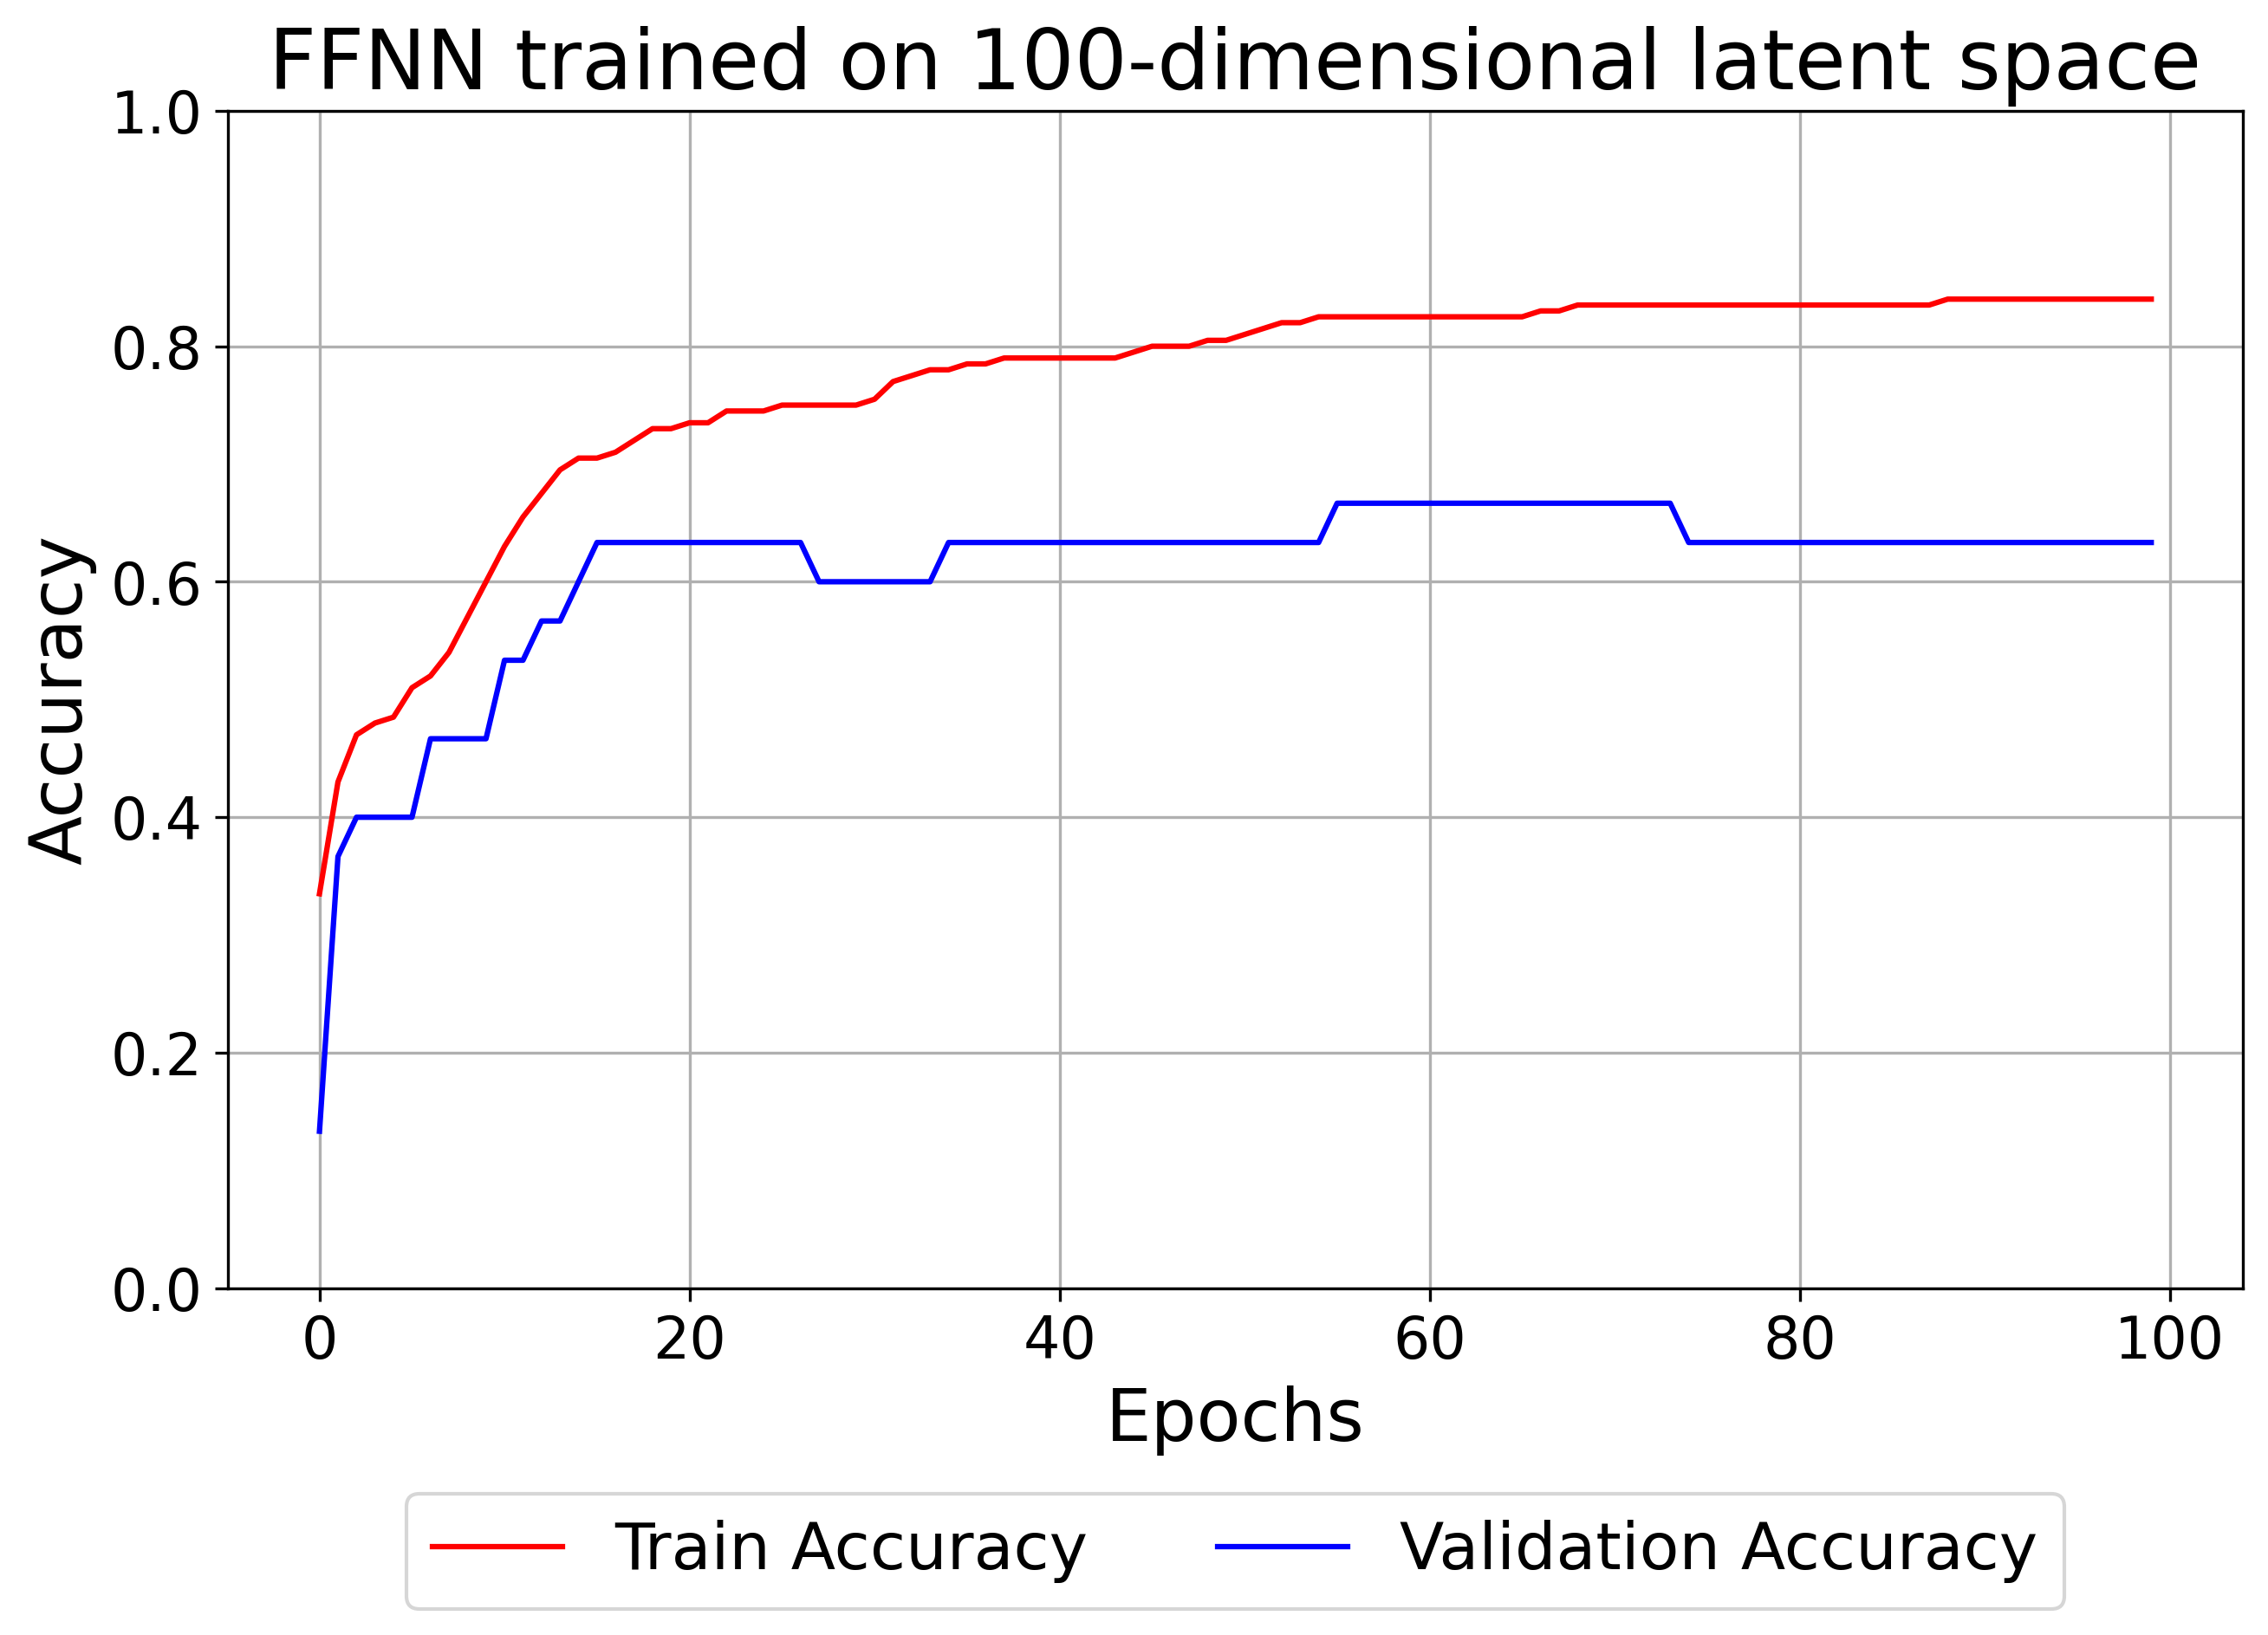
\includegraphics[width=0.33\textwidth]{02456_report/images/supp/learning_curve_subset1300_scvae100_H500.png}
    \caption{Learning curves from each FFNN model for the subset with 1,300 cells.}
    \label{sfig:lc1300}
\end{figure}



\begin{figure}[h!]
    \centering
    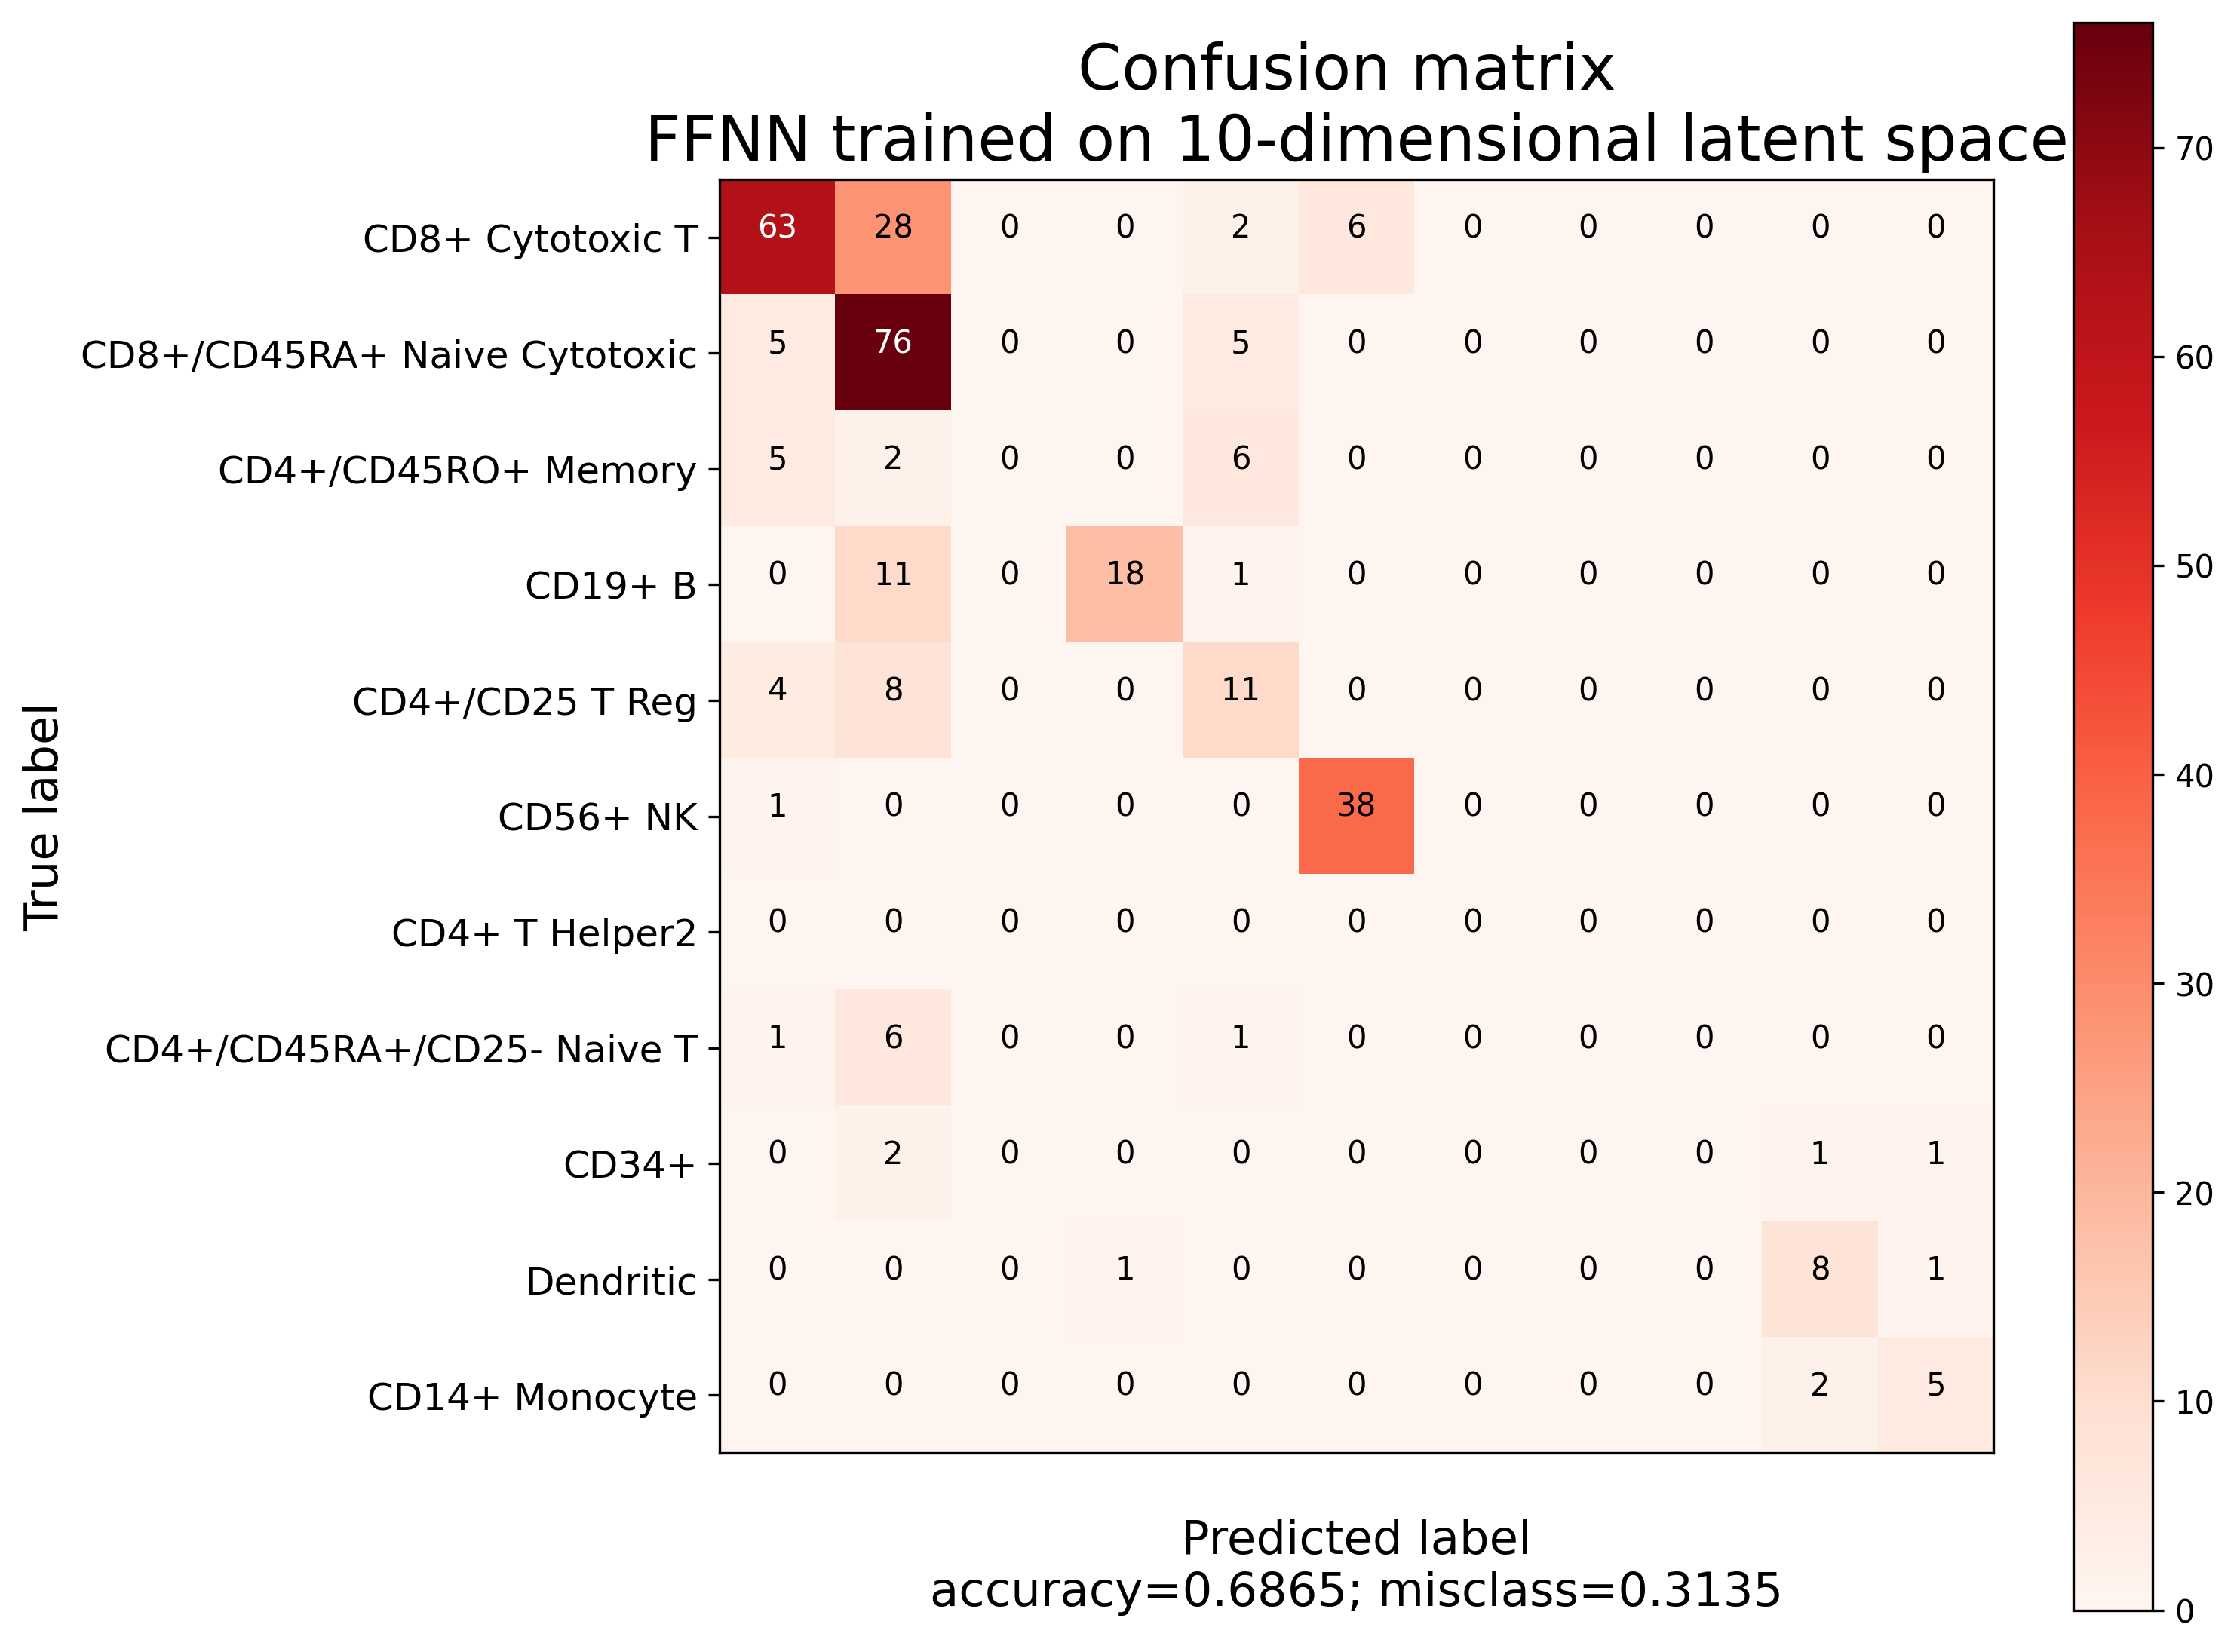
\includegraphics[width=0.33\textwidth]{02456_report/images/supp/confusion_matrix_subset15000_scvae10_H250.png}
    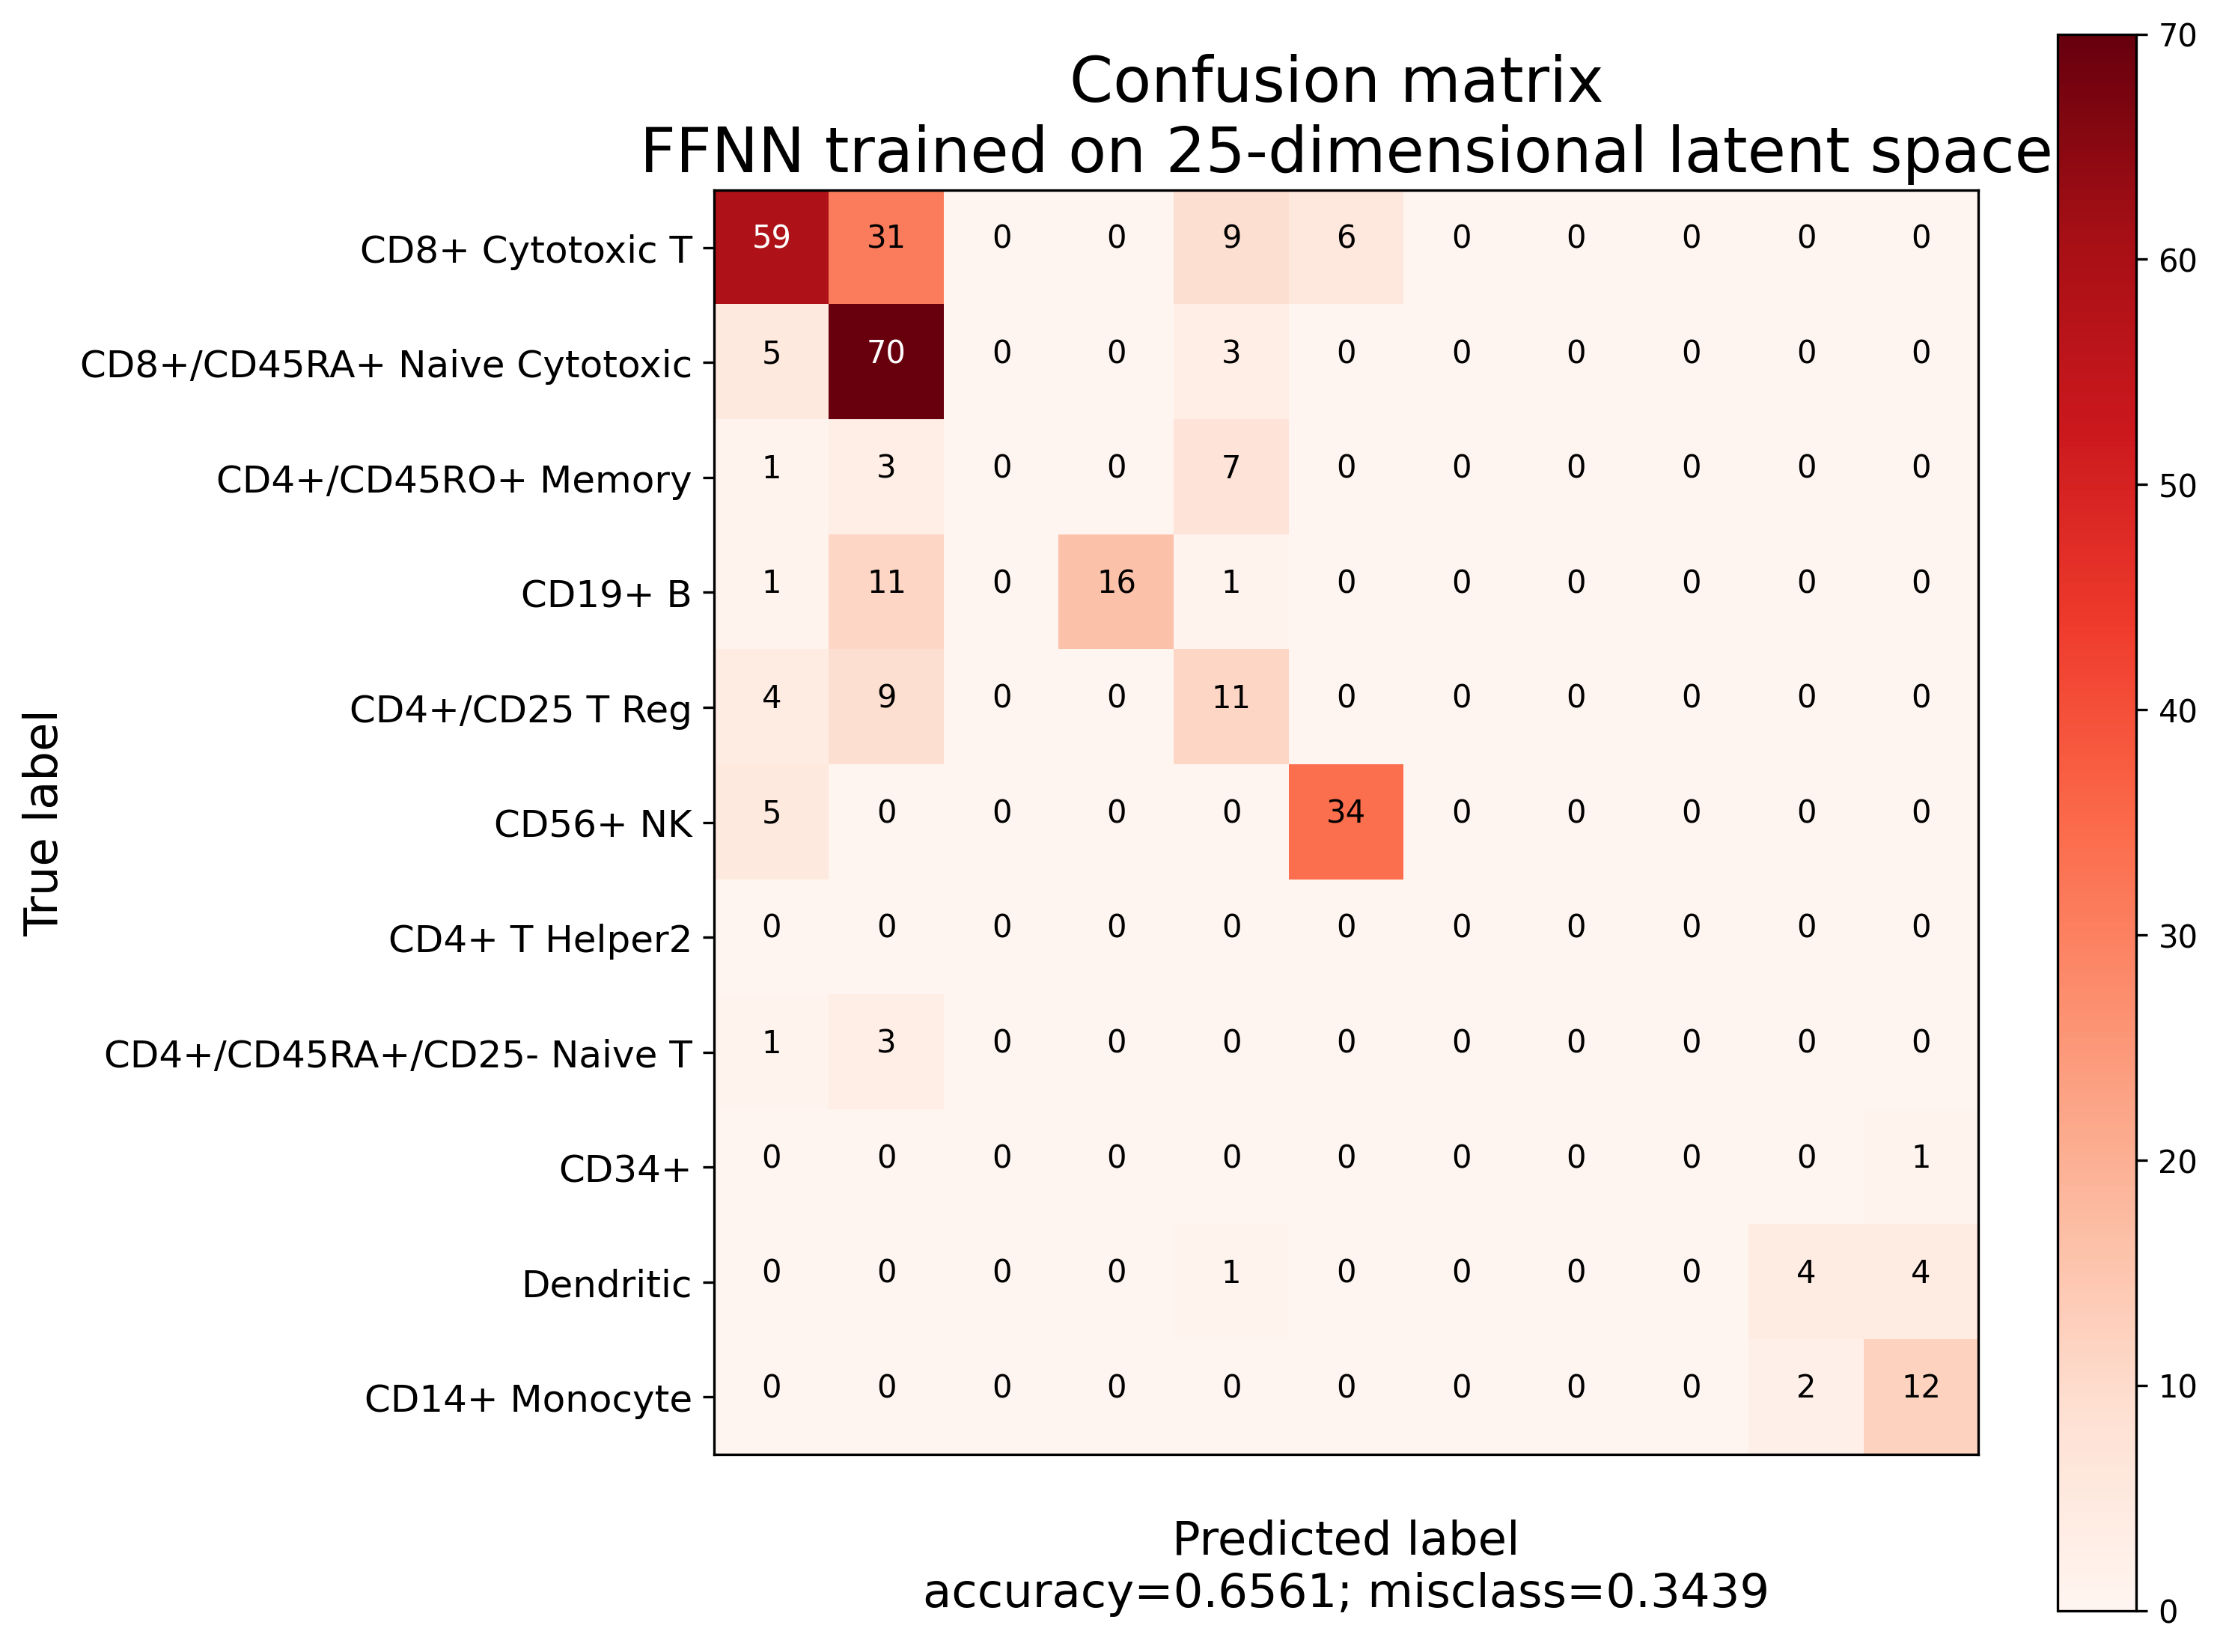
\includegraphics[width=0.33\textwidth]{02456_report/images/supp/confusion_matrix_subset15000_scvae25_H500.png}
    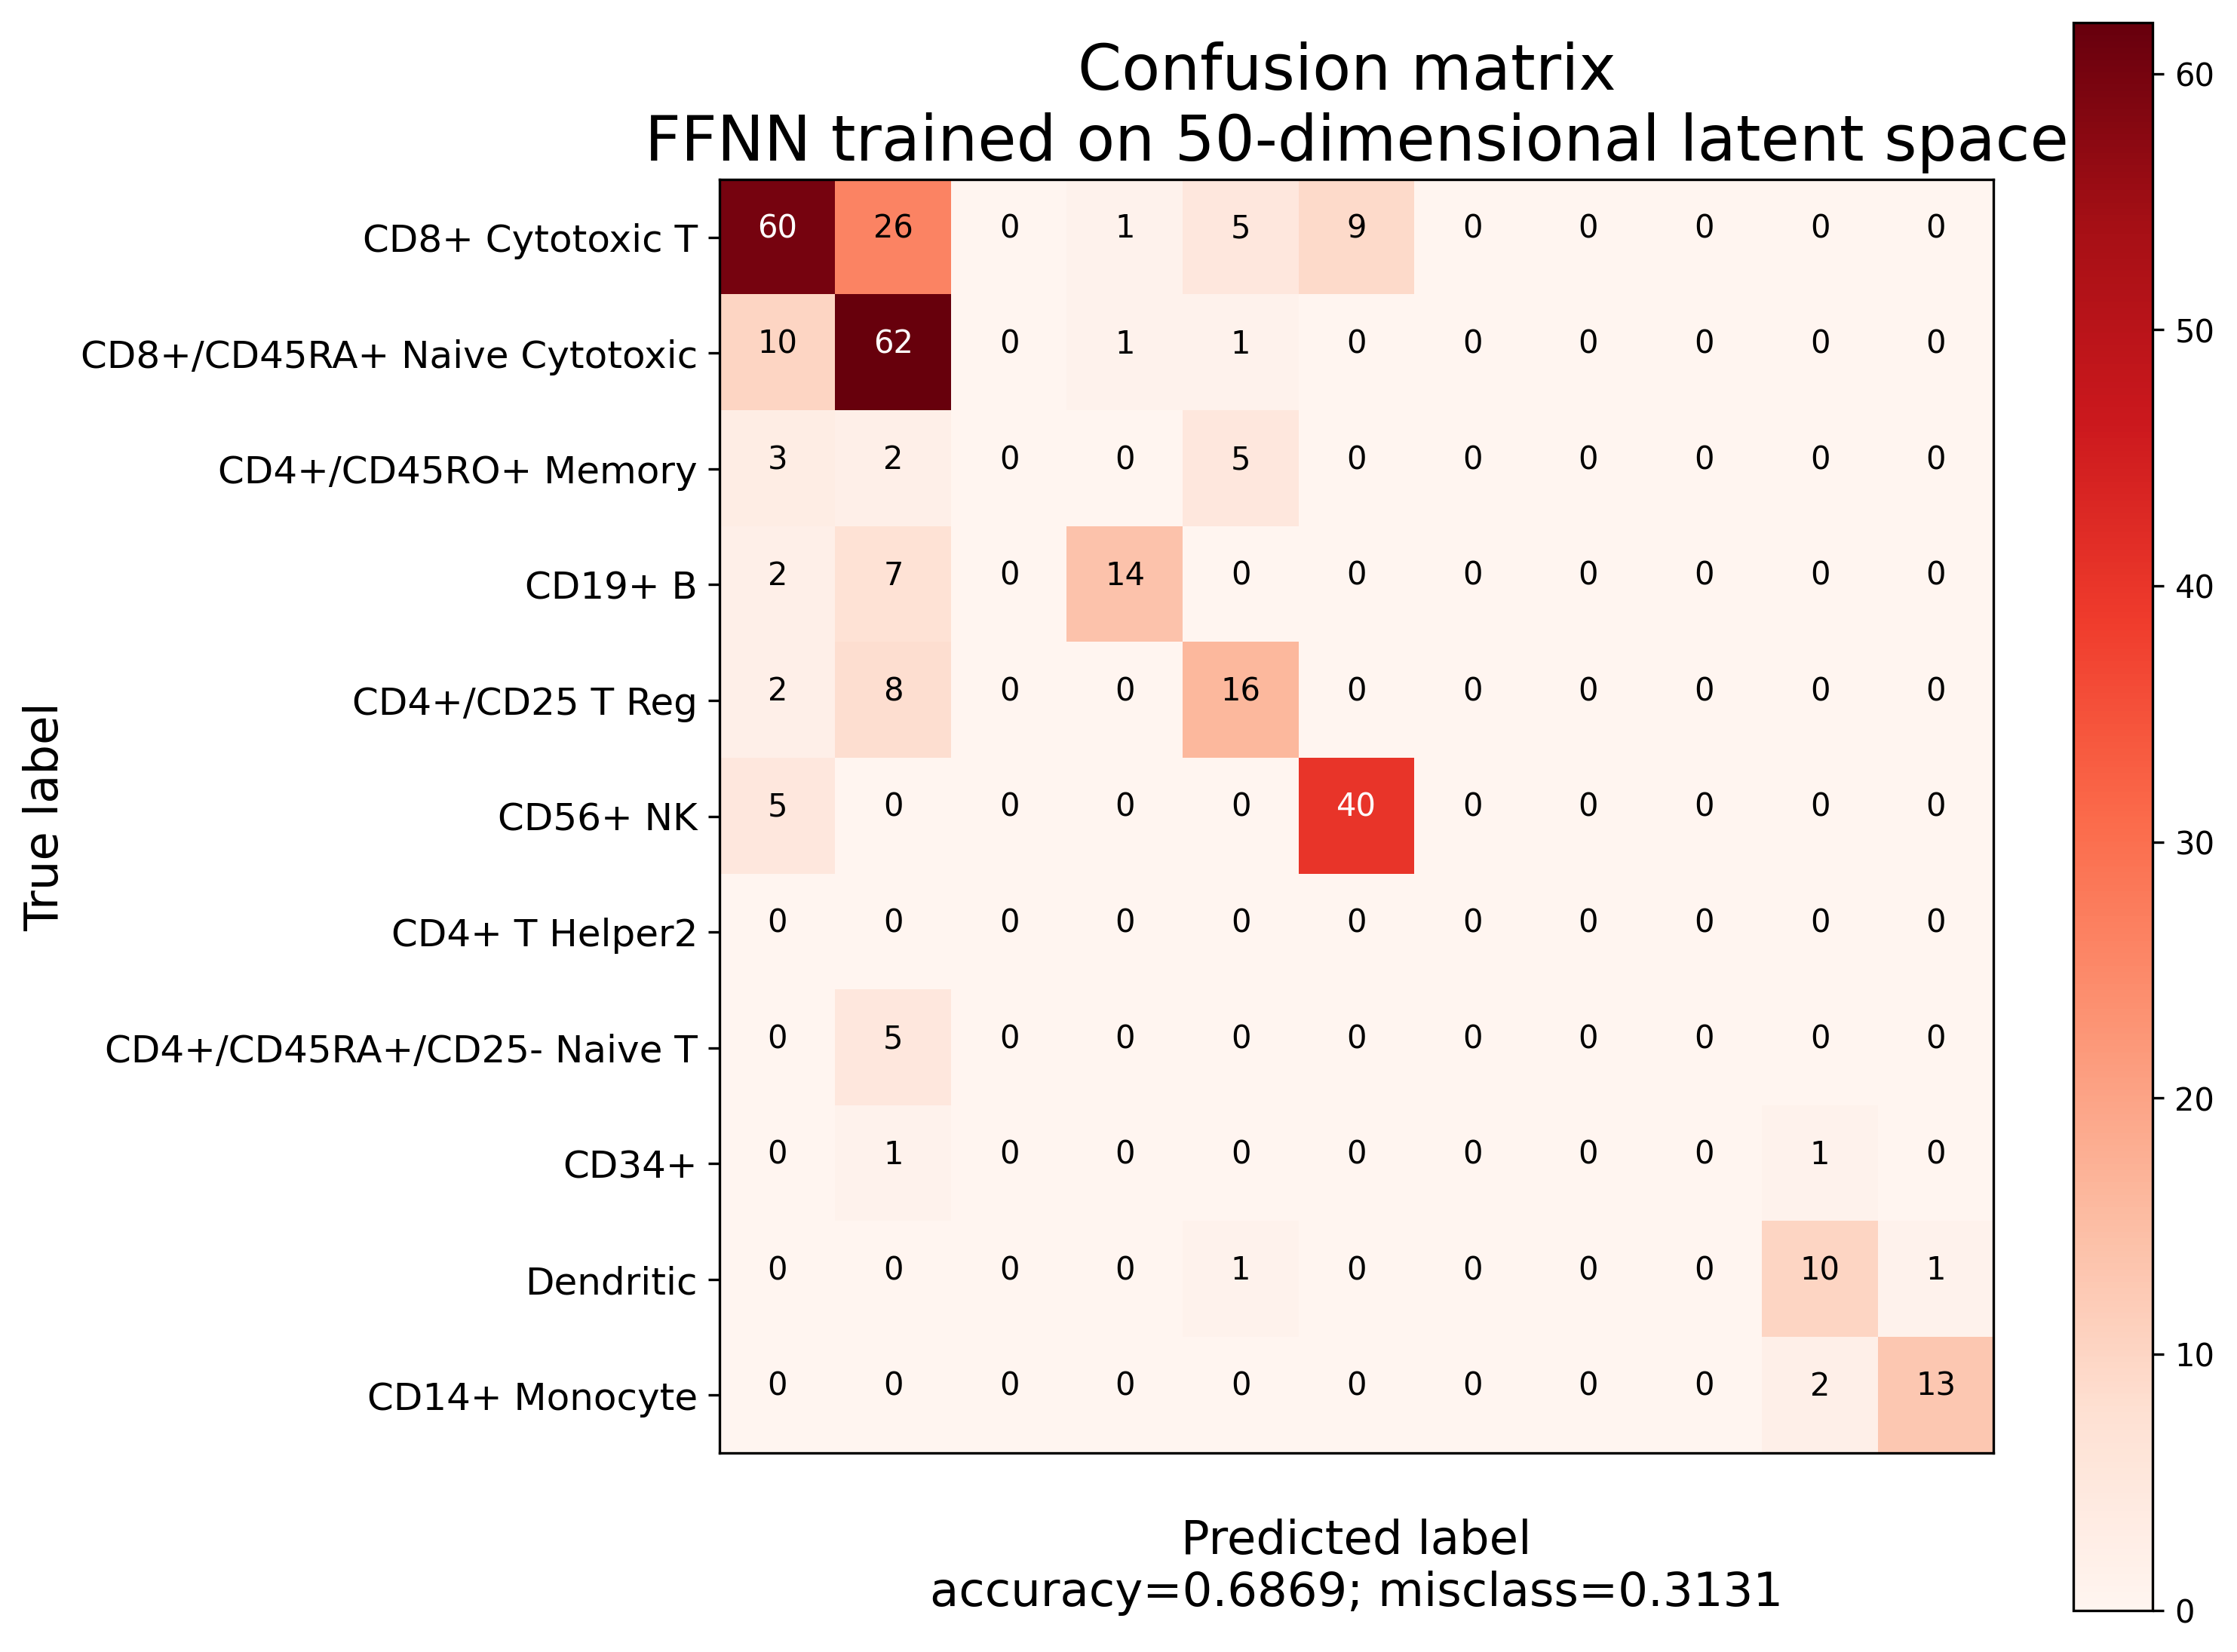
\includegraphics[width=0.33\textwidth]{02456_report/images/supp/confusion_matrix_subset15000_scvae50_H250.png}
    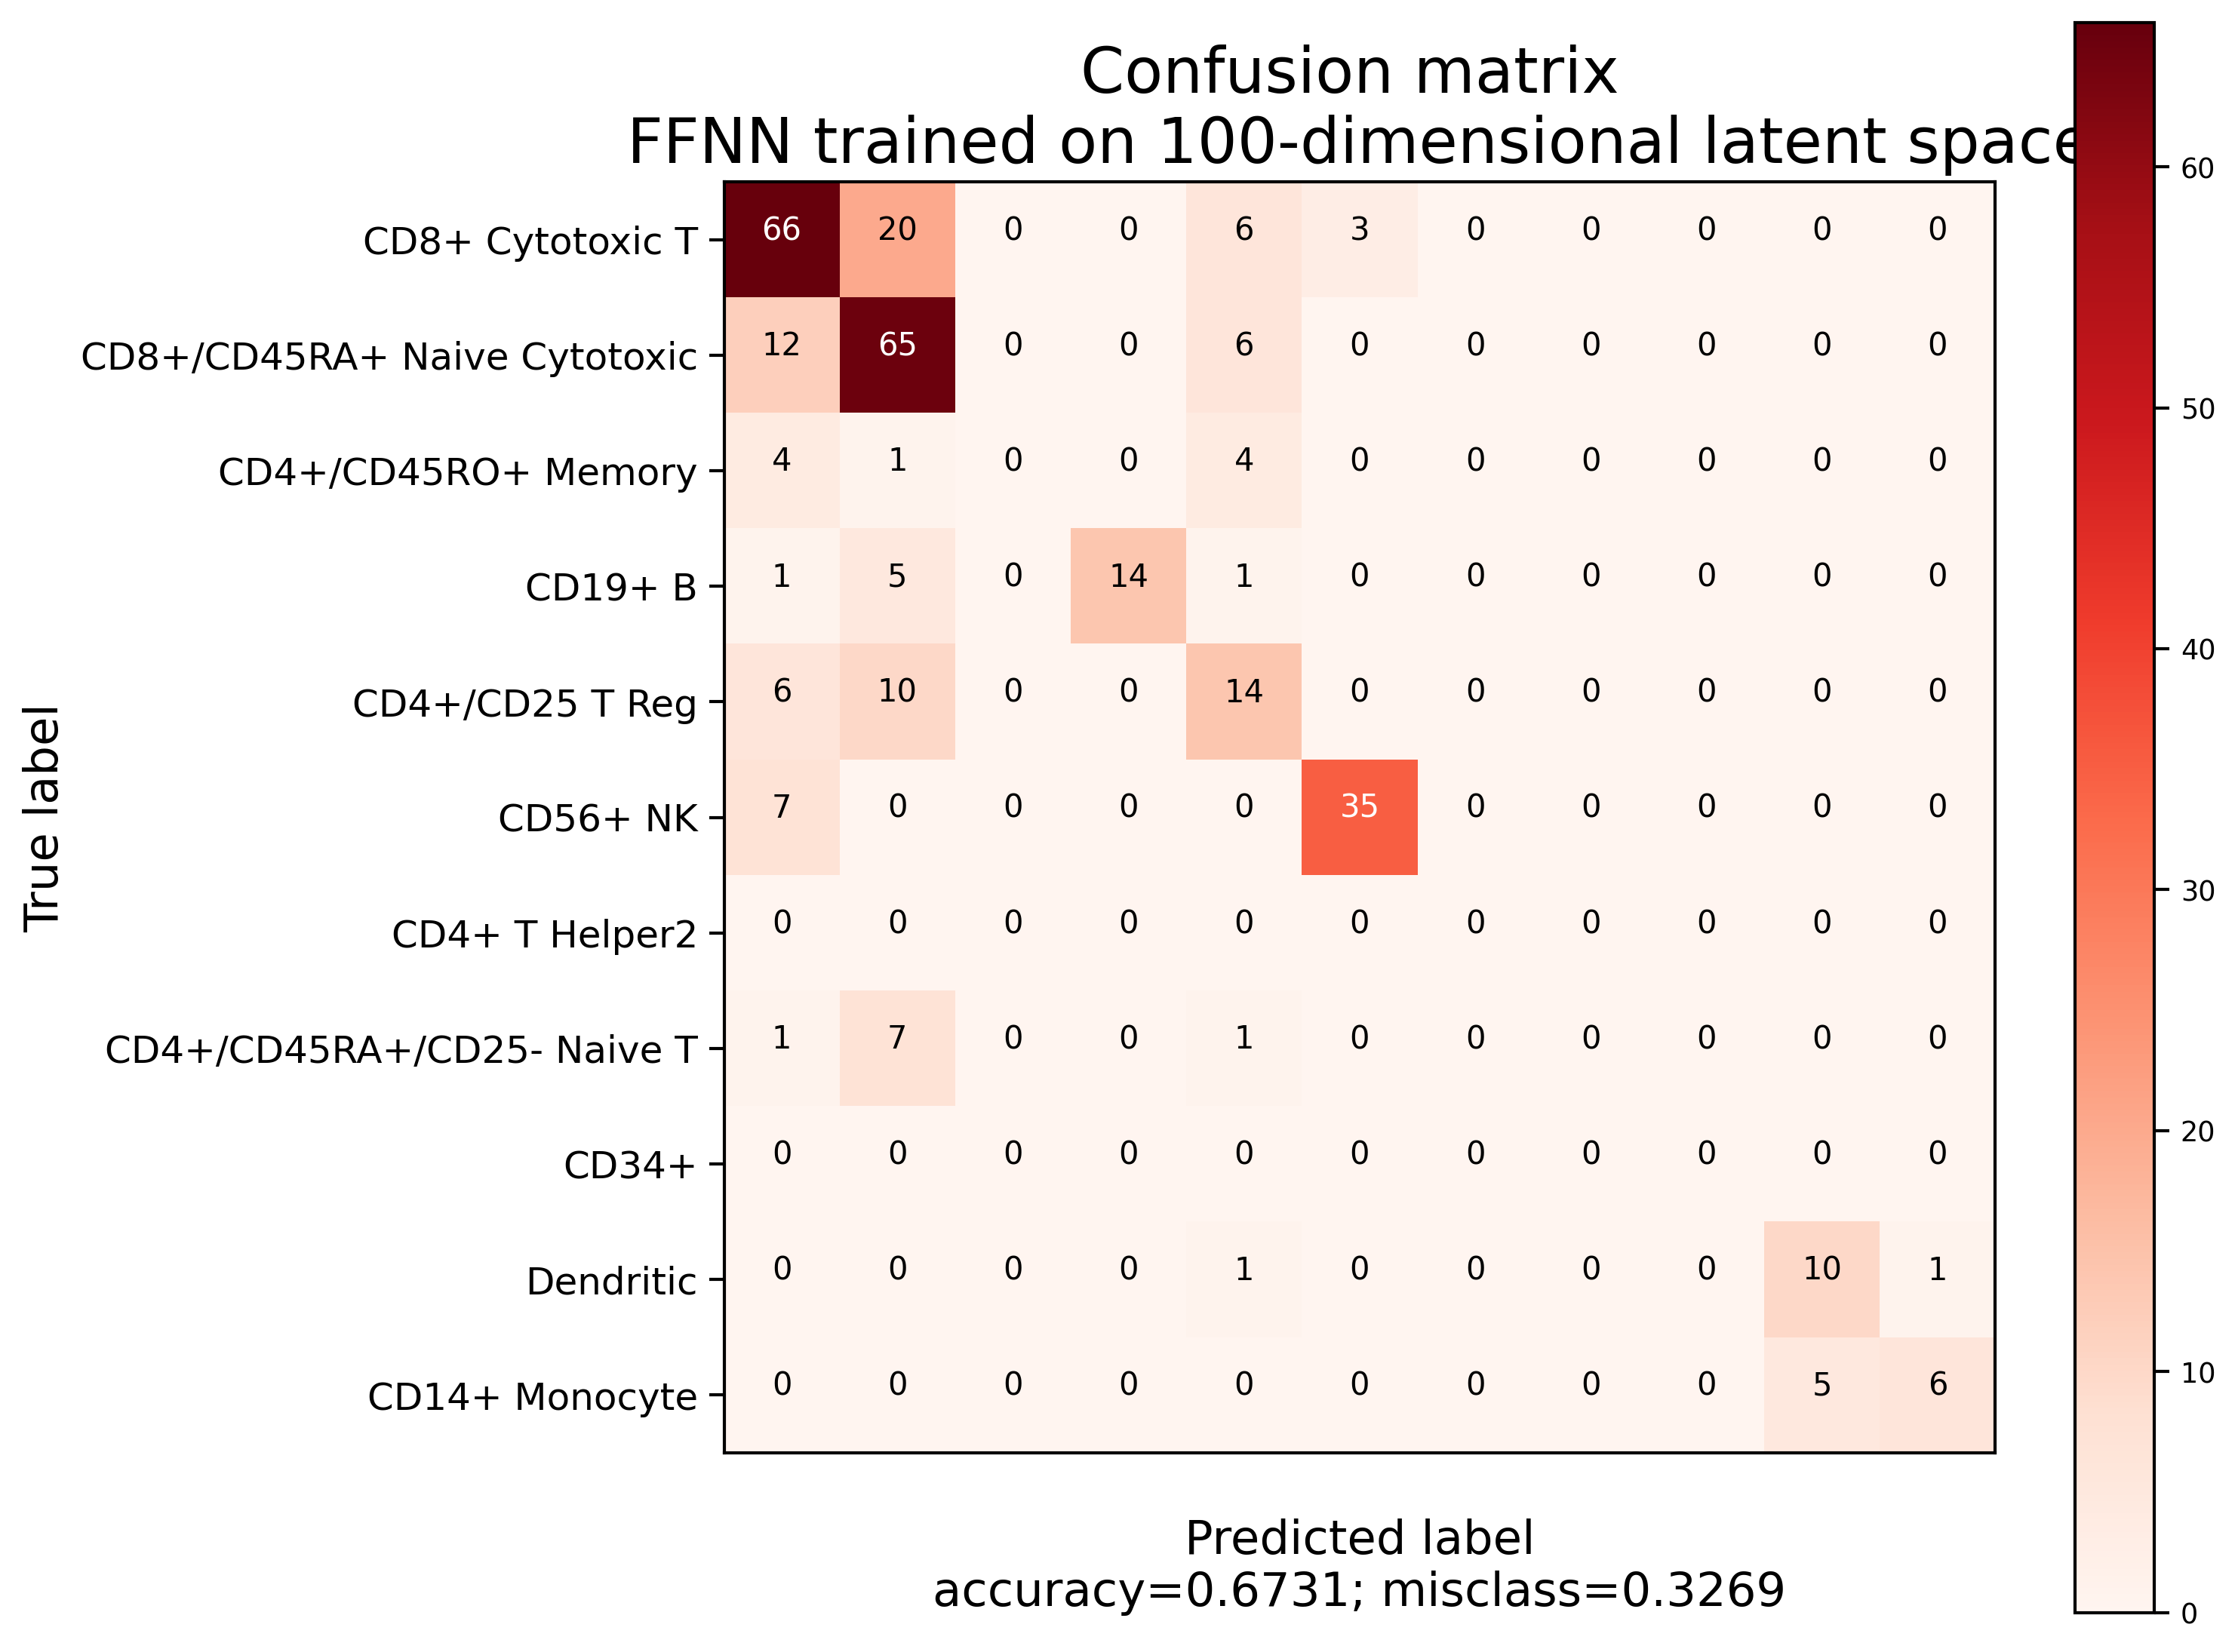
\includegraphics[width=0.33\textwidth]{02456_report/images/supp/confusion_matrix_subset15000_scvae100_H500.png}
    \caption{Confusion matrices from each FFNN model test set for the subset with 15,000 cells. }
    \label{sfig:confusions15000}
\end{figure}


\begin{figure}[h!]
    \centering
     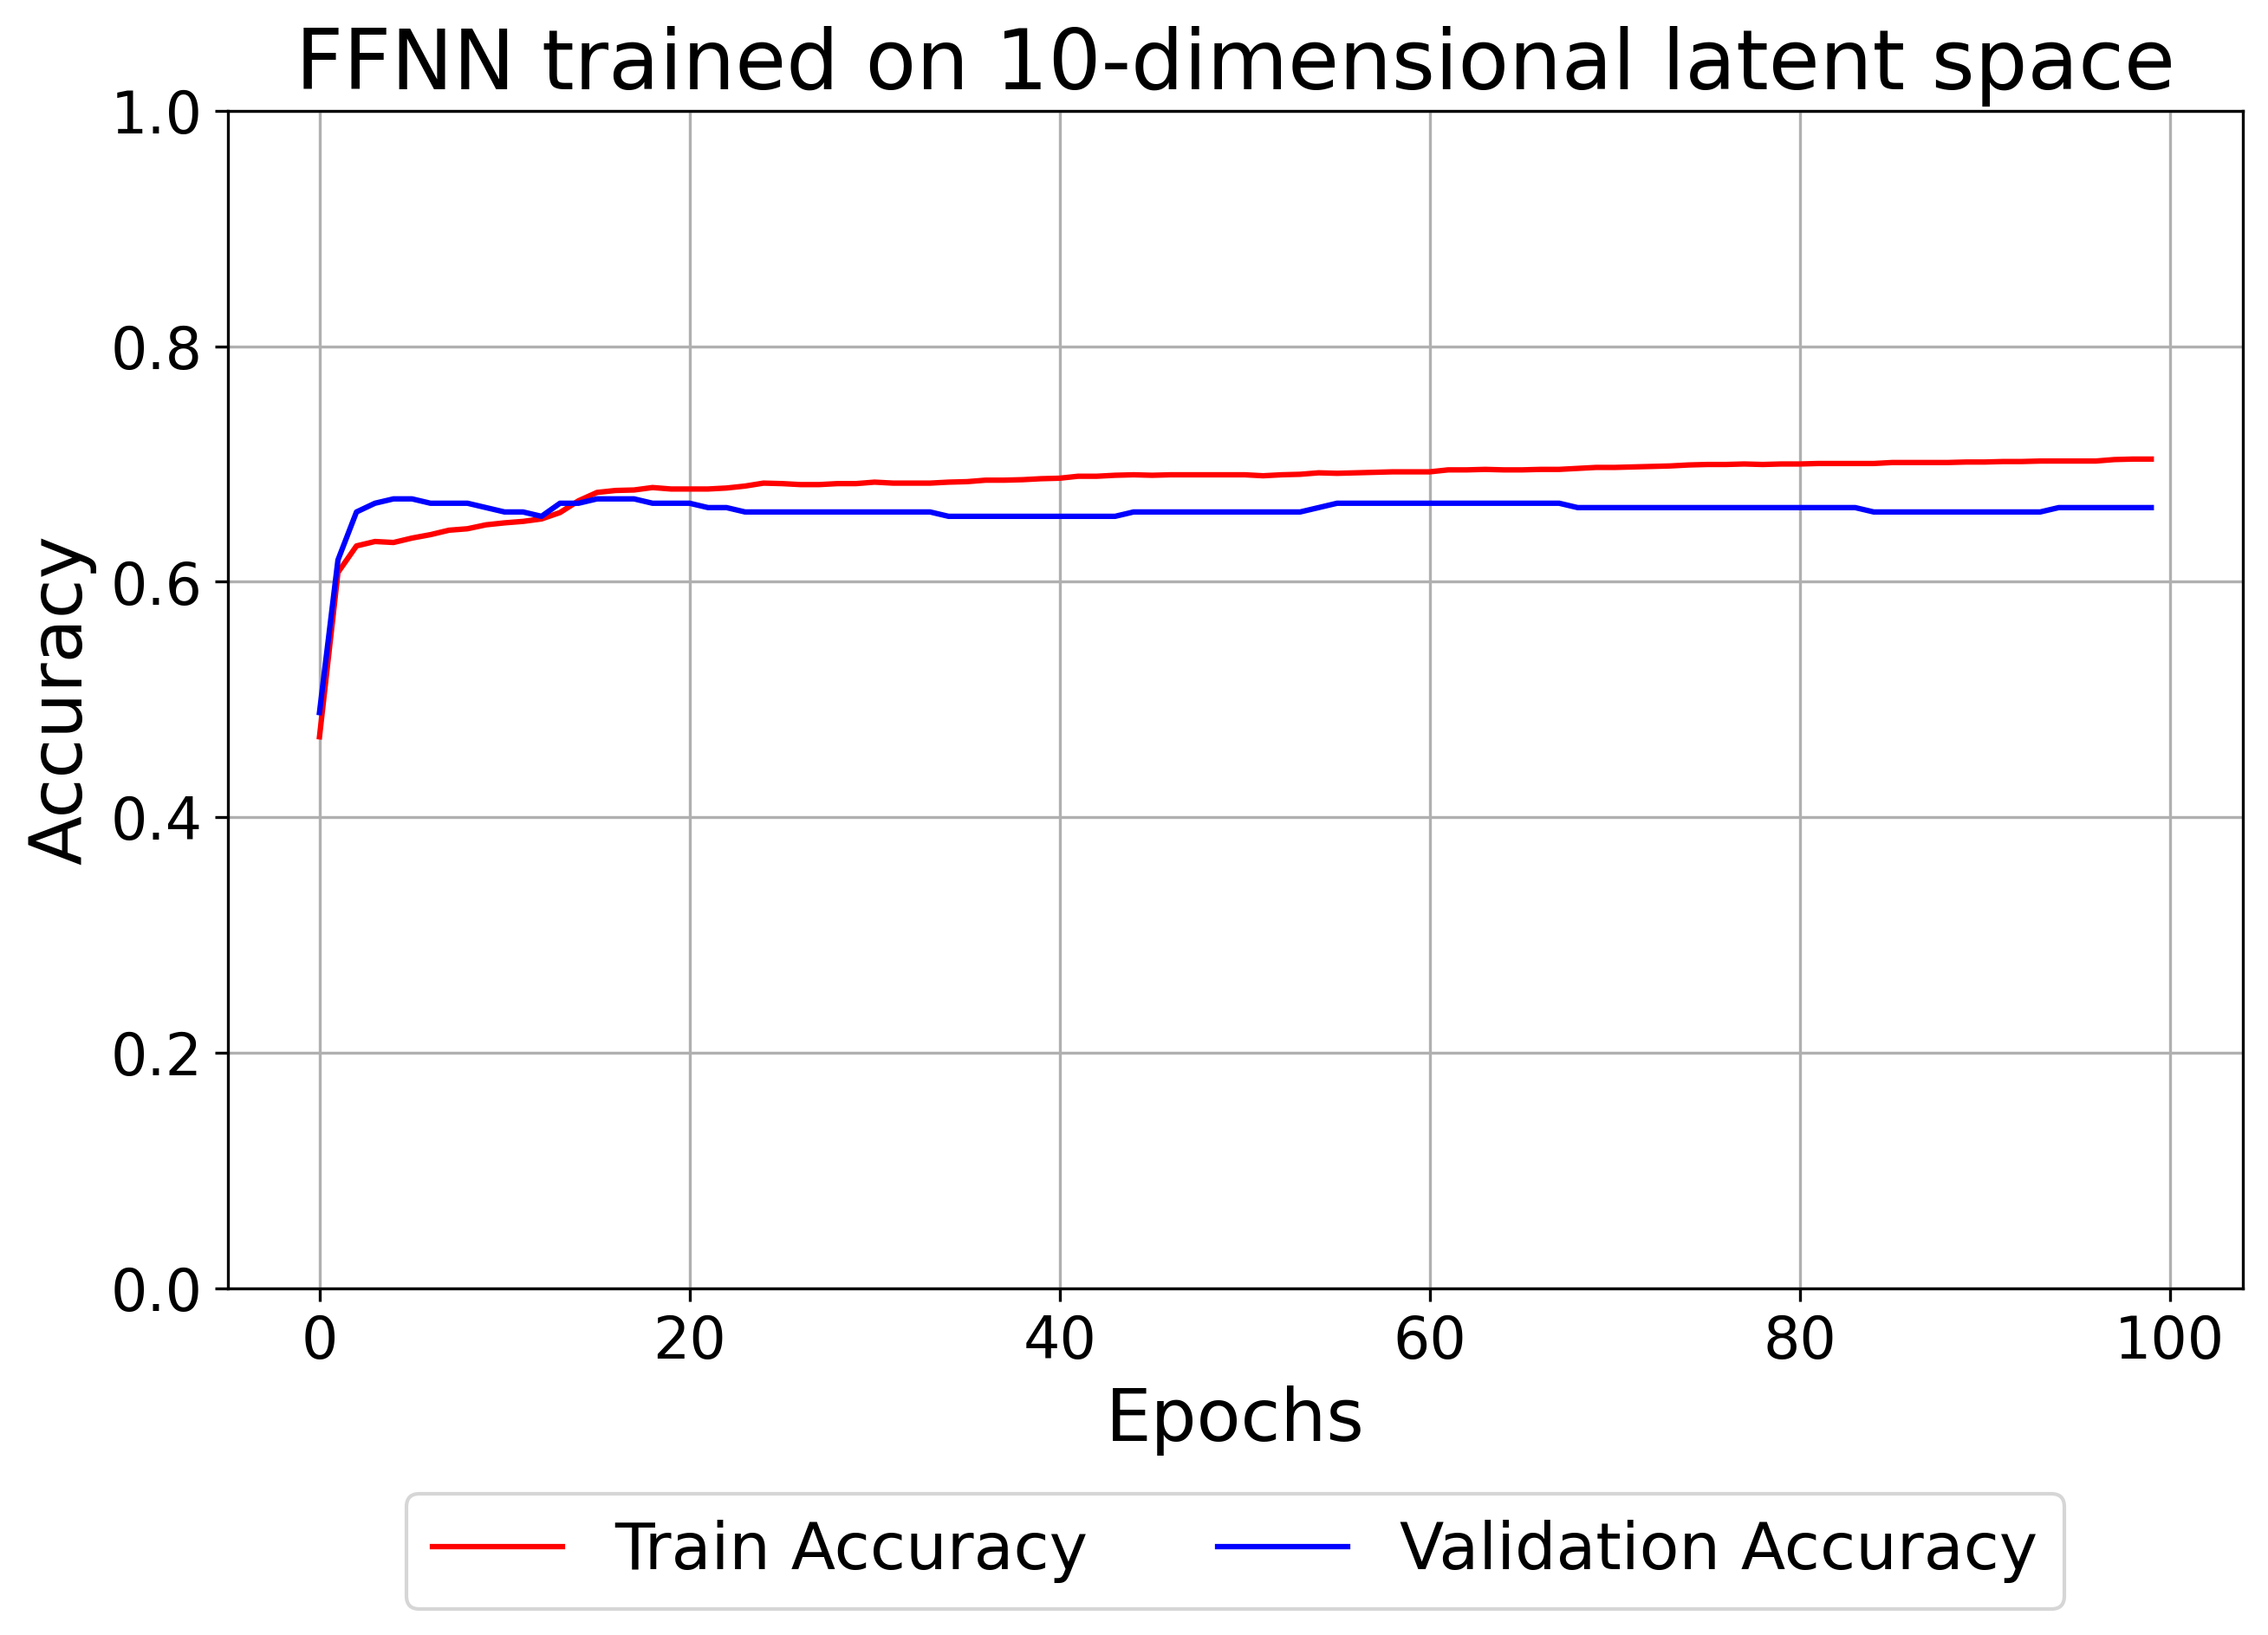
\includegraphics[width=0.33\textwidth]{02456_report/images/supp/learning_curve_subset15000_scvae10_H250.png}
    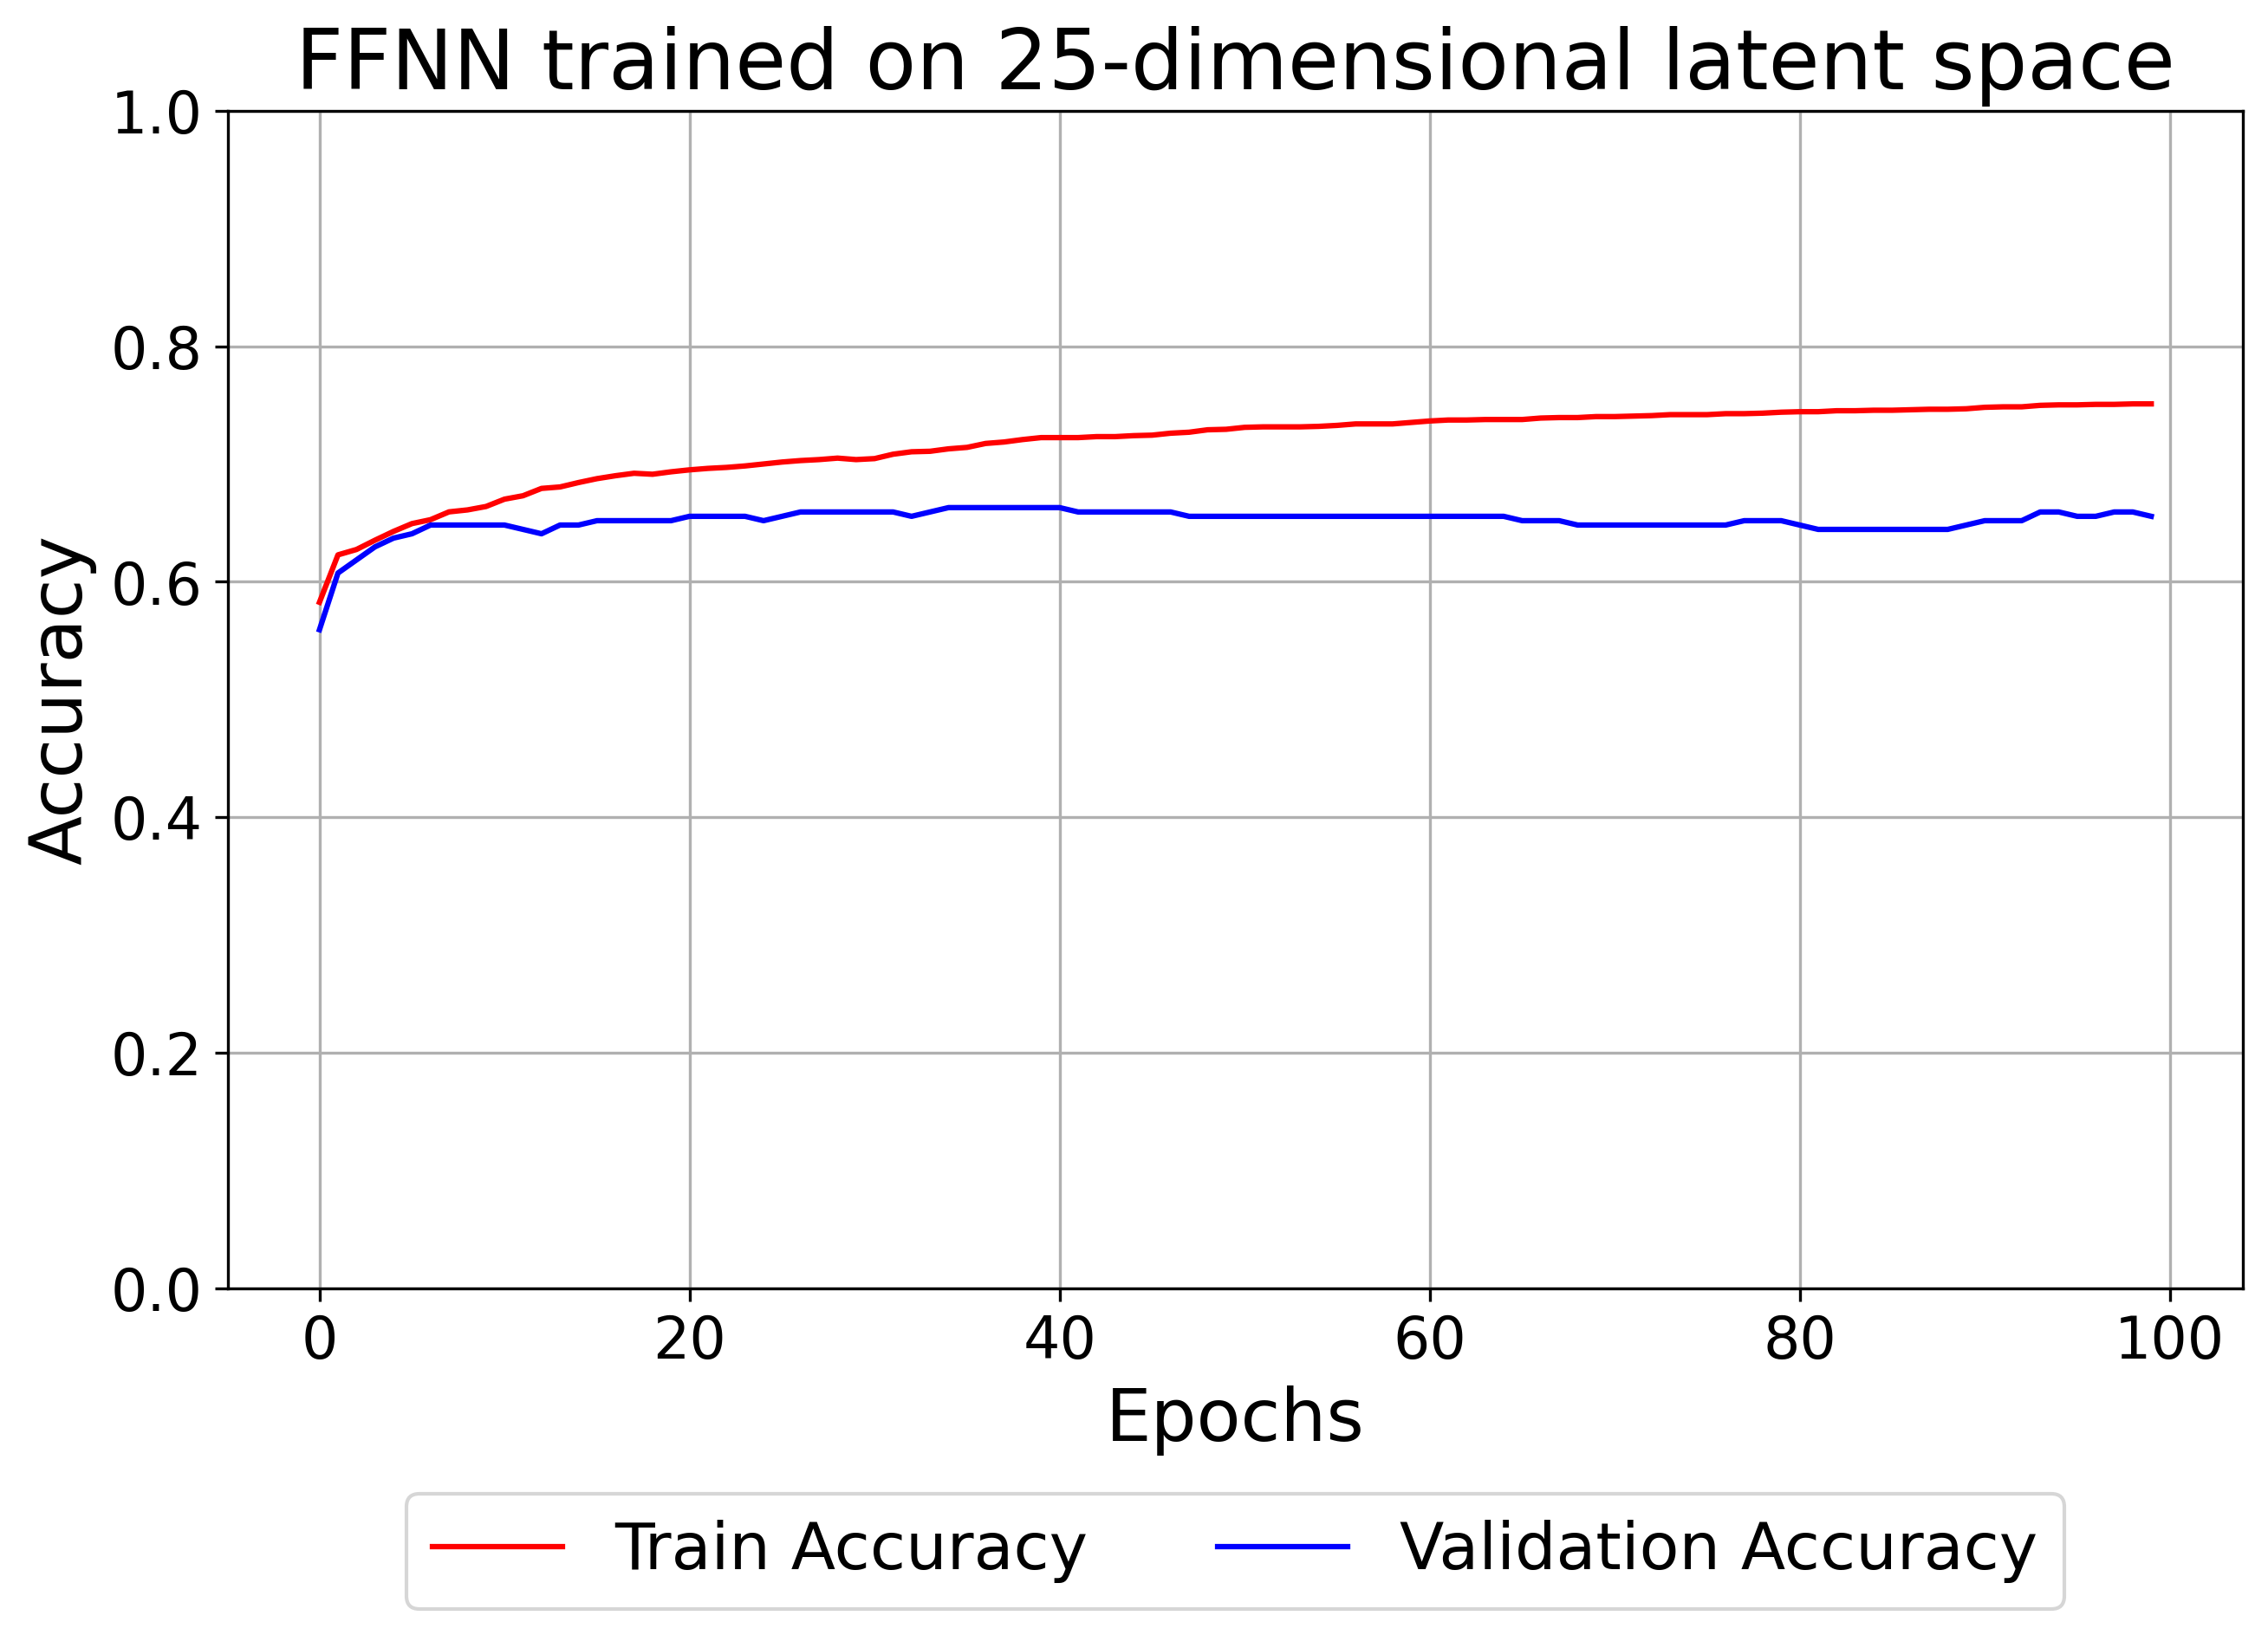
\includegraphics[width=0.33\textwidth]{02456_report/images/supp/learning_curve_subset15000_scvae25_H500.png}
    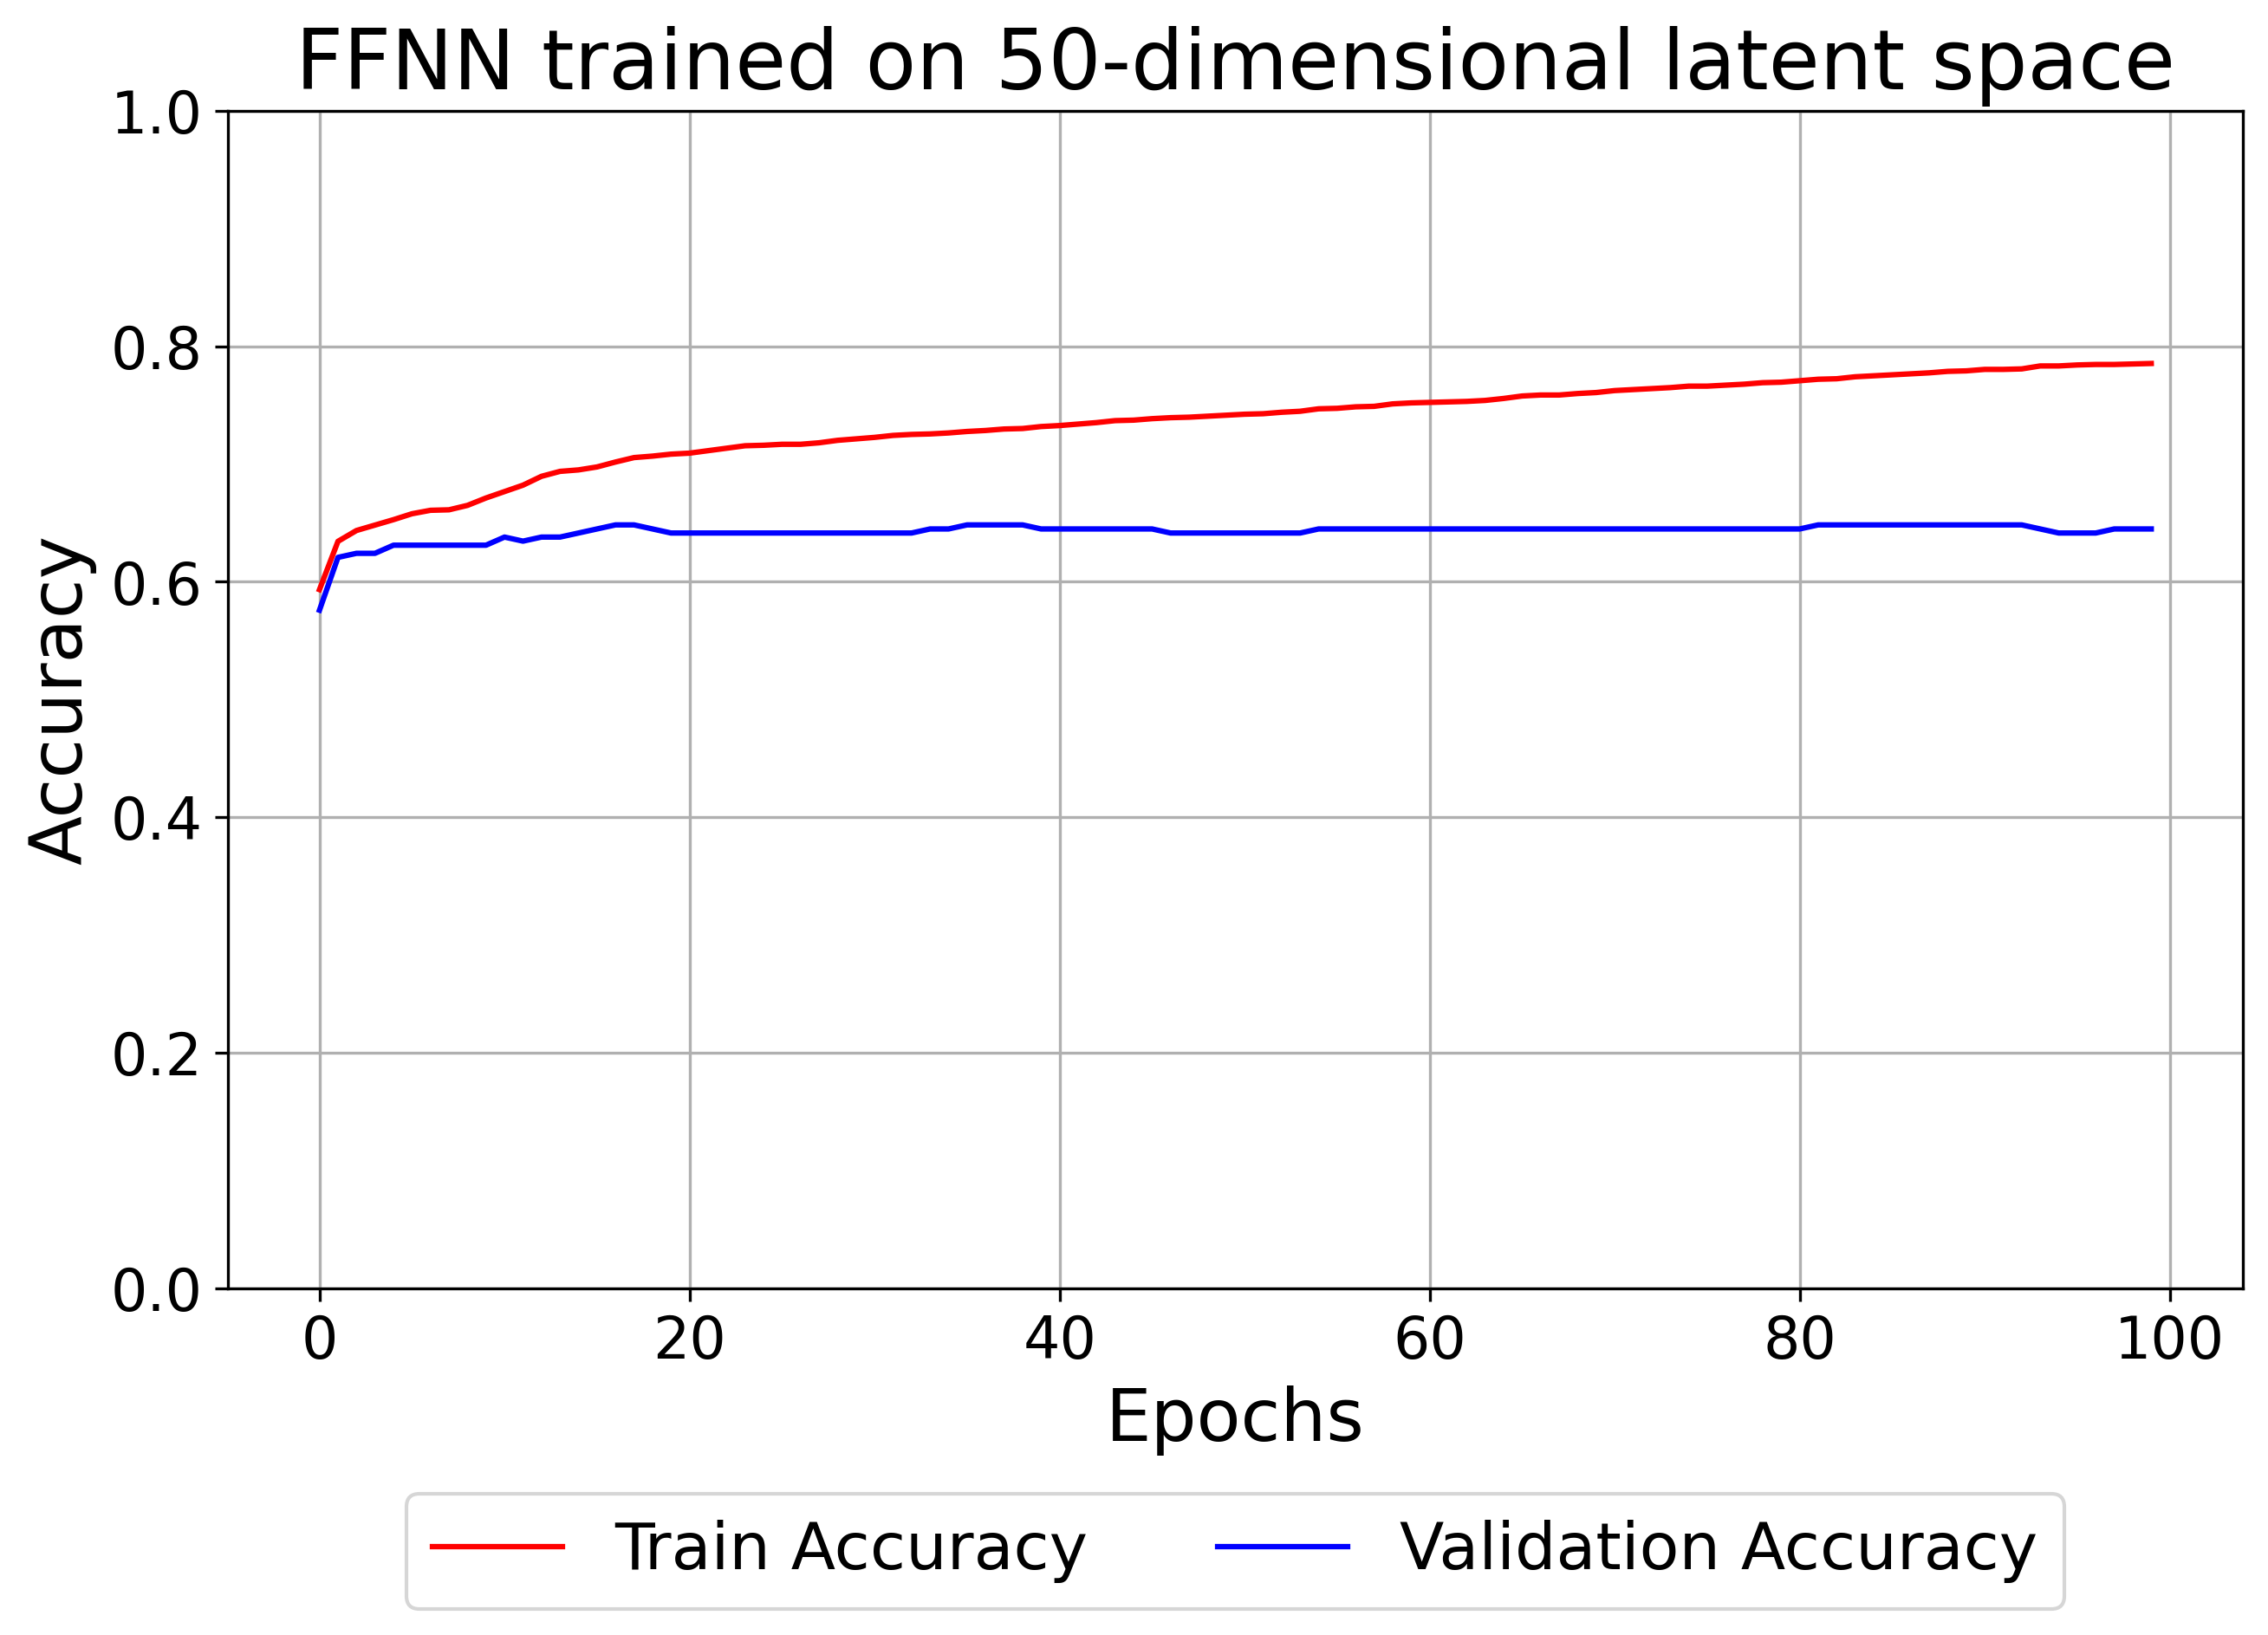
\includegraphics[width=0.33\textwidth]{02456_report/images/supp/learning_curve_subset15000_scvae50_H250.png}
    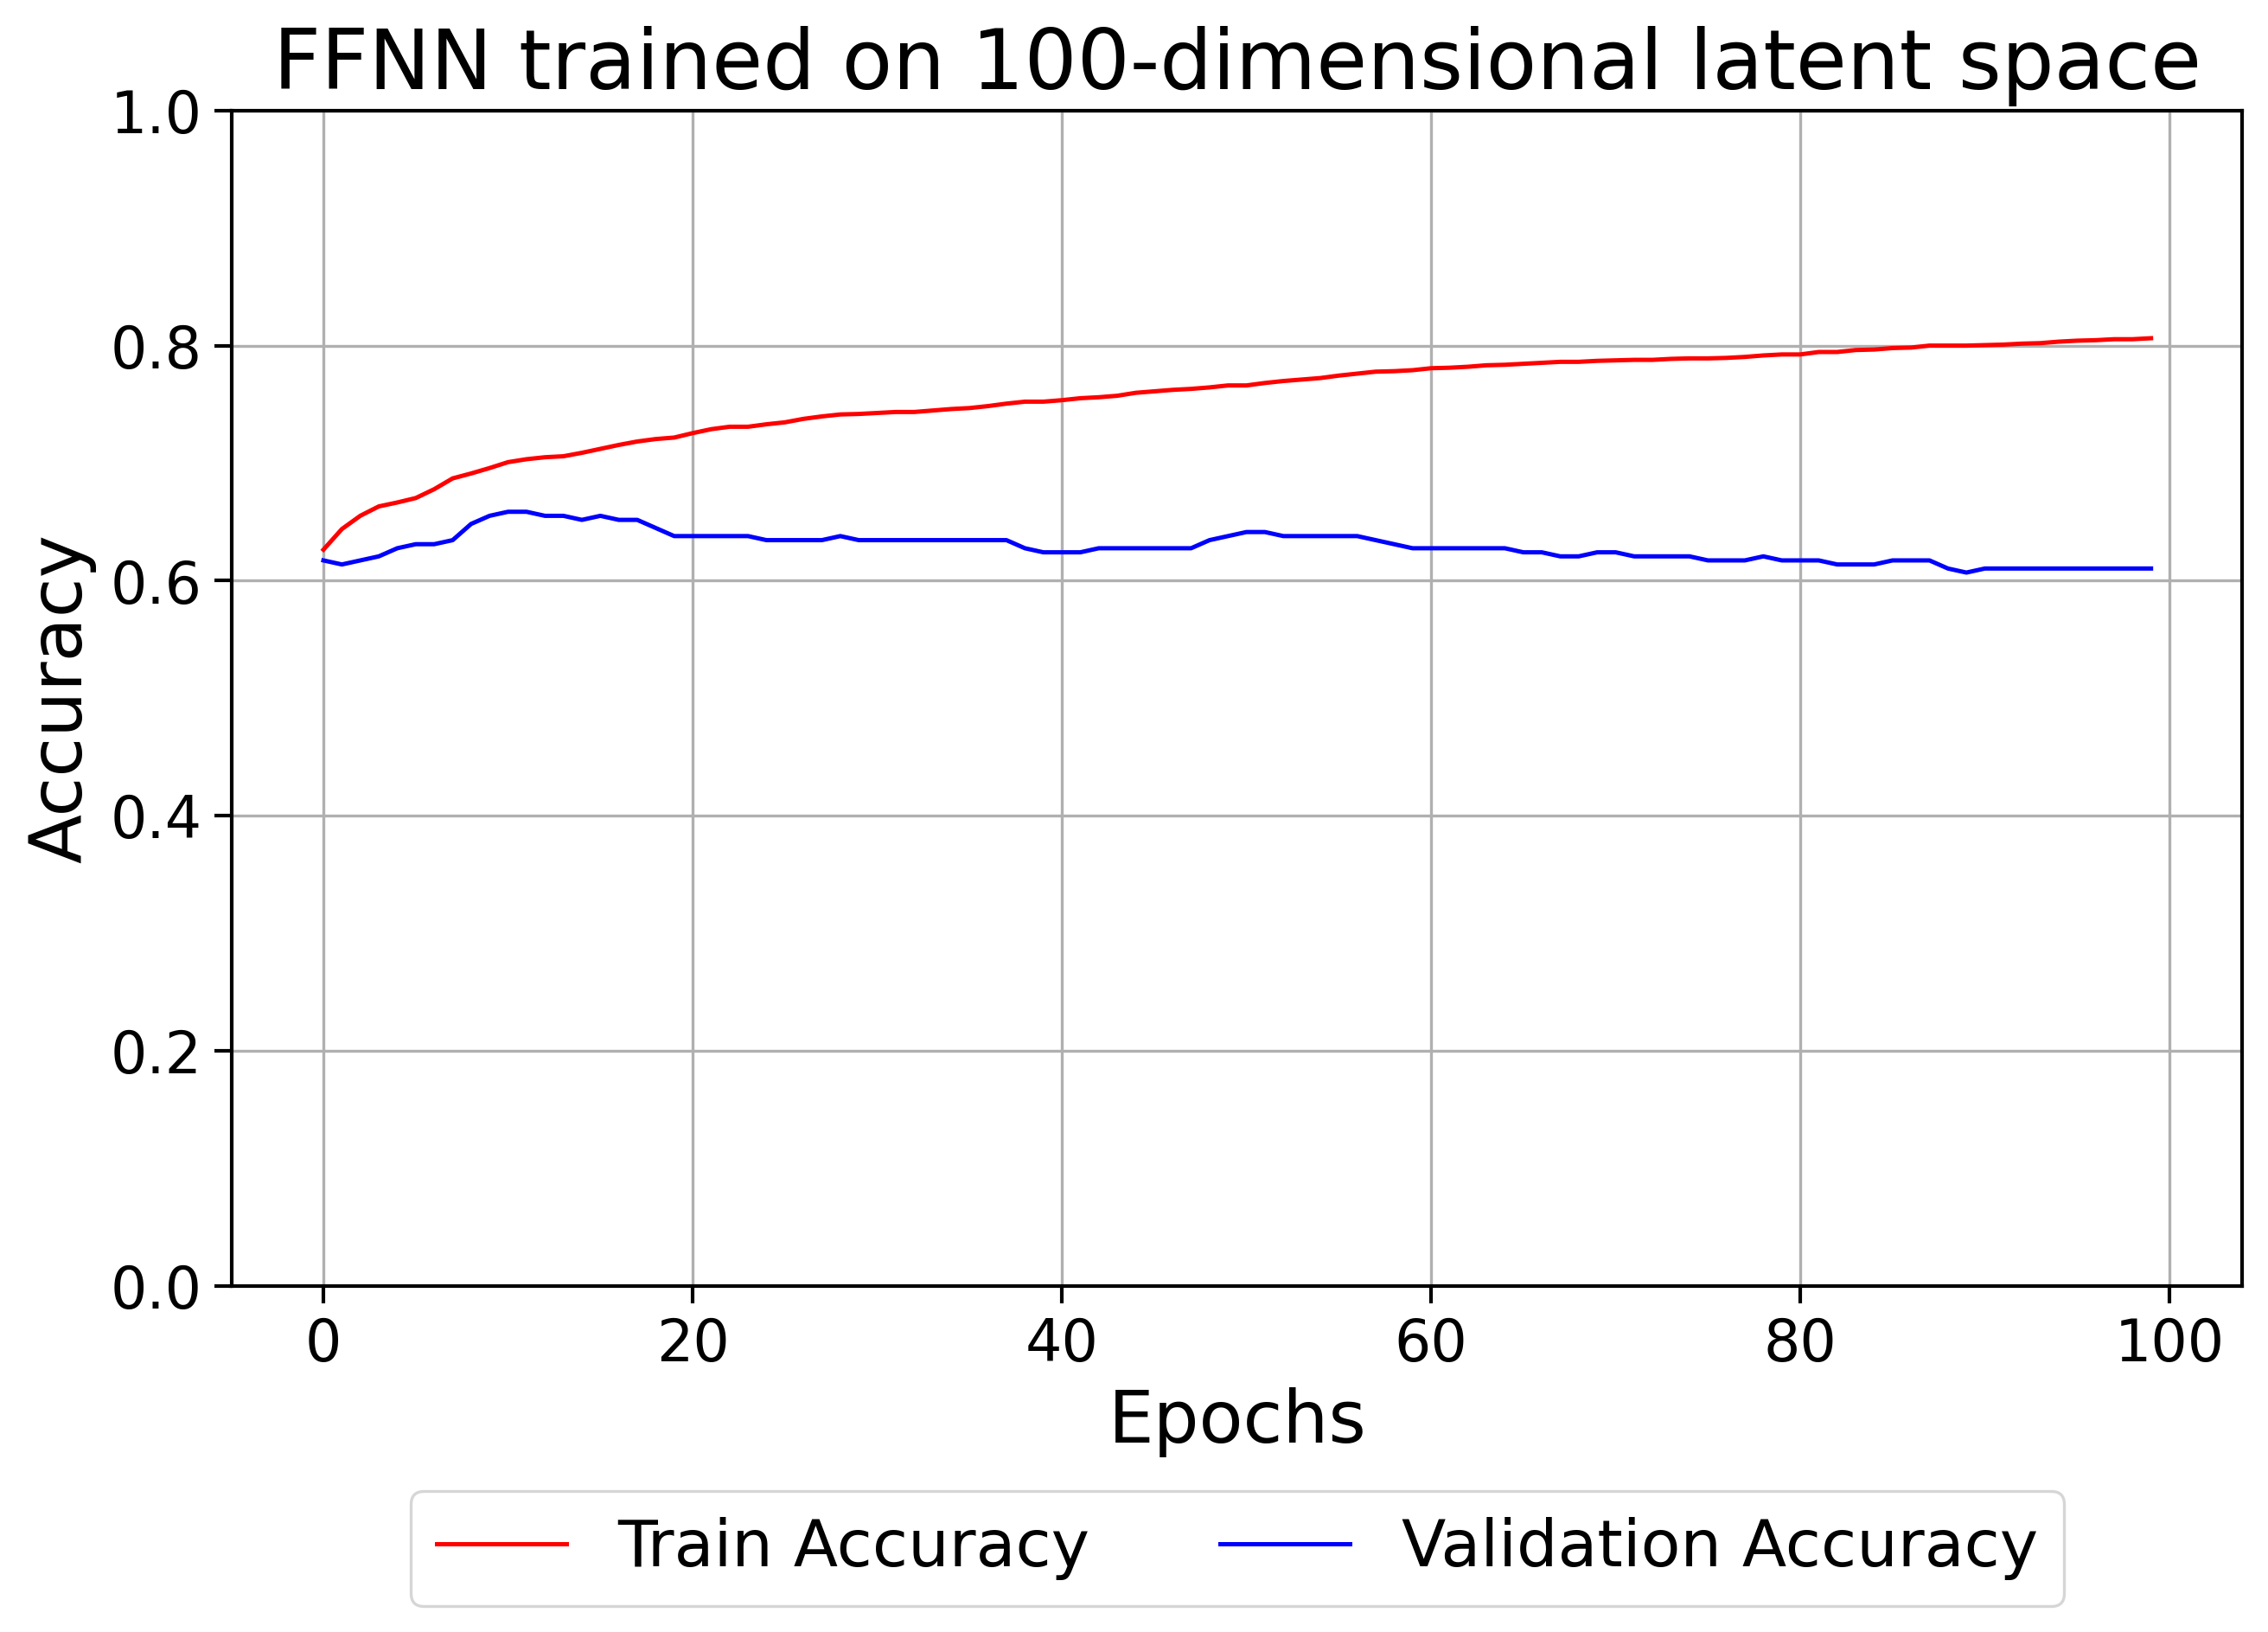
\includegraphics[width=0.33\textwidth]{02456_report/images/supp/learning_curve_subset15000_scvae100_H500.png}
    \caption{Learning curves from each FFNN model for the subset with 15,000 cells.}
    \label{sfig:lc15000}
\end{figure}






% class imbalance
\begin{figure}[h!]
    \centering
    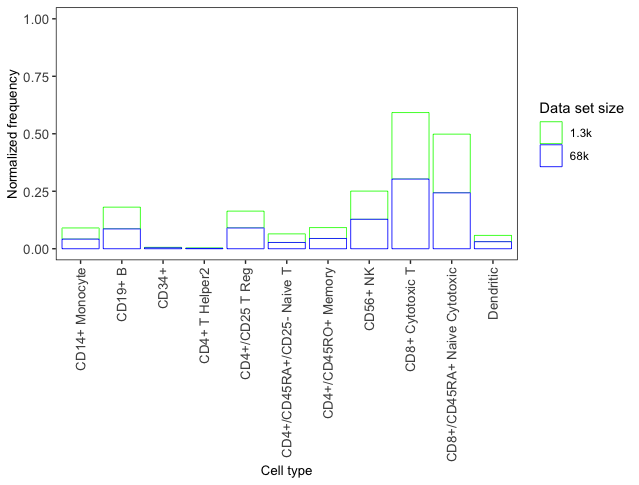
\includegraphics[width=0.80\textwidth]{02456_report/images/supp/Rplot02.png}
    \caption{Normalized number of cells per cell type in both the entire 10X-PBMC-68k data set and the 2\% subset that was used in the study.}
    \label{sfig:classes}
\end{figure} 


\end{document}
